\documentclass{scrartcl}
\usepackage{main}
\usepackage{flowchart}
%\section{Konfiguration}
% http://tex.stackexchange.com/questions/123374/reduce-space-at-the-top-using-maketitle
\title{\vspace{-2cm}Parallel realtime optimal control of a quadcopter}
\subtitle{Projektreport: Advanced Topics in High Performance Scientific Computing}
\author{Benedikt König}
\begin{document}
\maketitle

\section{Einleitung}
\subsection{Motivation}
Die autonome Steuerung eines Fluggerätes ist durch die starken und schnellen Änderungen der Umgebung - besonders durch die Windeinflüsse - eine schwierige Aufgabe. Daher können die optimalen Steuerungssignale nicht vor dem Start berechnet werden. Die passende Steuerungstrategie muss während des Fluges gefunden werden. Hierzu werden Methoden von real-time Optimierung und Strategien von model predictive control kombiniert, um einen Quadrocopter zu steuern.  

\subsection{Übersicht}
Für das dynamische System des Quadrocopters wird die optimale Steuerungsstrategie gesucht, um Unsicherheiten in der Umgebung und im Modell, wie zum Beispiel Windeinflüsse, auszugleichen. In diesem Kontext wird zwischen den Steuerungssignalen $u$ und States $x$ unterschieden. Eine Beziehung zwischen beiden wird durch die ODE $\dot{x(t)}=f(x(t), u(t))$ erreicht. Das Ziel ist es, eine Steuerung $u$ zu finden, welche eine gegebene Kostenfunktion $J$, die die ODE und deren Randwertbedingungen als Nebenbedingung besitzt, zu minimieren. D.h.
\begin{align}
	\min_{x, u} J(x(t), u(t)) \text{ u.d.N. } \dot{x(t)} = f(x(t), u(t)) \text{ und } x(0) = x_0\text{, } x(1) = x_1
\end{align}

Es existieren verschiedene Techniken, um dieses unendlich dimensionale Optimierungsproblem zu lösen. Diese indirekten Methoden sind aber nicht realtime fähig. Daher wird in diesem Projekt die direkte Methode benutzt: Dabei wird das unendliche dimensionale Optimierungsproblem durch ein endlich nichtlineares Problem ersetzt, um die Steuerungssignale sowie die Zustände zu approximieren. Für die Approximation wird das sogenannte multiple shooting Verfahren verwendet, welches anschließend mit Hilfe der SQP - Methode gelöst wird. Bei den gegebenen Modell- und Umgebungsparametern erreicht diese Methode eine gute numerische Approximationen für $u$ in der Kürze der Zeit. Der Ansatz dieses Projektes ist angelehnt an die Methoden, welche entwickelt worden sind von Diehl et al. \cite{Diehl2001, Diehl2002}\\
\\
Für die Implementierung des Projektes wurden folgende Bereiche berücksichtigt: Modellierung des Quadrocoptermodelles, Implementierung der Diskretierung und der SQP - Methode sowie der Realtime Ansatz.

\subsection{Entwicklung und Entscheidungen}
Das Projekt ``Parallel realtime optimal control of a quadcopter'' ist aus den Case Studies for Nonlinear Optimization des Sommersemesters 2015 entstanden. Dazu mussten wir in einem Team, bestehend aus Philipp Fröhlich, Simon Kick, Annika Stegie und mir (Benedikt König) einen Quadrocopter mit Hilfe der Ansätze von Diehl et al.\cite{Diehl2001, Diehl2002} in Echtzeit optimieren. Wir entschieden uns für die Entwicklungsumgebung MATLAB, da alle mit jenen vertraut waren und sich besonders das Debuggen als einfach herausgestellt hatte. Nachdem Erfolg des Projektes ``rtopt'' kam der Wunsch auf, dieses weiterzuführen und die Ergebnisse in eine konkurrenzfähige Umgebung zu transformieren. Zunächst wurde von mir versucht das Projekt unter FORTRAN zu übersetzten, dies ist leider aufgrund von Compilierverfügbarkeit (Stand: 31.03.2016 ist PGI CUDA Fortran Compiler der einzige CUDA Compiler für Fortran -> teuer) gescheitert. Für den zweiten Versuch wurde das Projekt nun in ``c'' erstellt. Dafür sprachen unter anderem die hohe Plattformverfügbarkeit, Performance und benutzte OpenSource Projekte. Dies waren unter anderem das OpenSource Projekt ``SuiteSparse'' mit dem Paket ``CSparse'' von Timothy A. Davis \cite{davis2006direct} und das Projekt CVODE von Alan C. Hindmarsh \cite{Hindmarsh1996}. Das Paket CSparse beinhaltet eine Vielzahl von Sparsematrixoperationen, sowie Direktlöser (lu, qr, ..) von Gleichungssystemen mit Sparsematrizen. CVODE hingegen löst Anfangswertprobleme von gewöhnlichen Differentialgleichungen. Im Laufe des Projektes musste besonders das Paket ``CSparse'', welches auf den compressed sparse column(csc) Format basiert, angepasst und erweitert werden. Zudem stellte sich heraus, dass das Schreiben von Testfunktionen in ``C'' eine Herausforderung war und die Kombination aus den MATLAB Projekt ``rtopt'' und ``c''-Projekt eine schnellere Alternative darstellte. Dabei wurden, durch die vorhandenen und korrekt funktionieren MATLAB - Funktionen, Daten generiert und mit den neuen Funktionen des ``c''- Projektes verglichen. 
% -*- root: ../main.tex -*-
\subsection{Quadrocopterdynamik}
In der Literatur gibt es verschiedene dynamische Modelle für Quadrocopter mit unterschiedlicher Komplexität. In diesem Projekt wurde das Modell von \cite{LQR2013} verwendet. 
\subsection{Herleitung}
Für die Herleitung des Modelles hat sich als passender physikalischer Ansatz die Newton'schen - Bewegungsgleichungen bewährt. \\\\

Dazu lässt sich der Multikopter in drei Körpergruppen ($B_0, B_1, B_2$) einteilen: Bezugssystem (Startpunkt), ``nicht rotierende Körper'' (Grundplatte, Arme, Controller, Batterie, etc) und ``rotierende Körper'' (Motor, Rotor, Rotorschraube). In der Abbildung \ref{fig:schubkraefte} lassen sich die Schubkräfte $F_1, ... F_4$, wirkend im jeweiligen rotierenden System $B_{M1}, ..., B_{M2}$, erkennen.
\begin{figure}[ht]
  \centering
  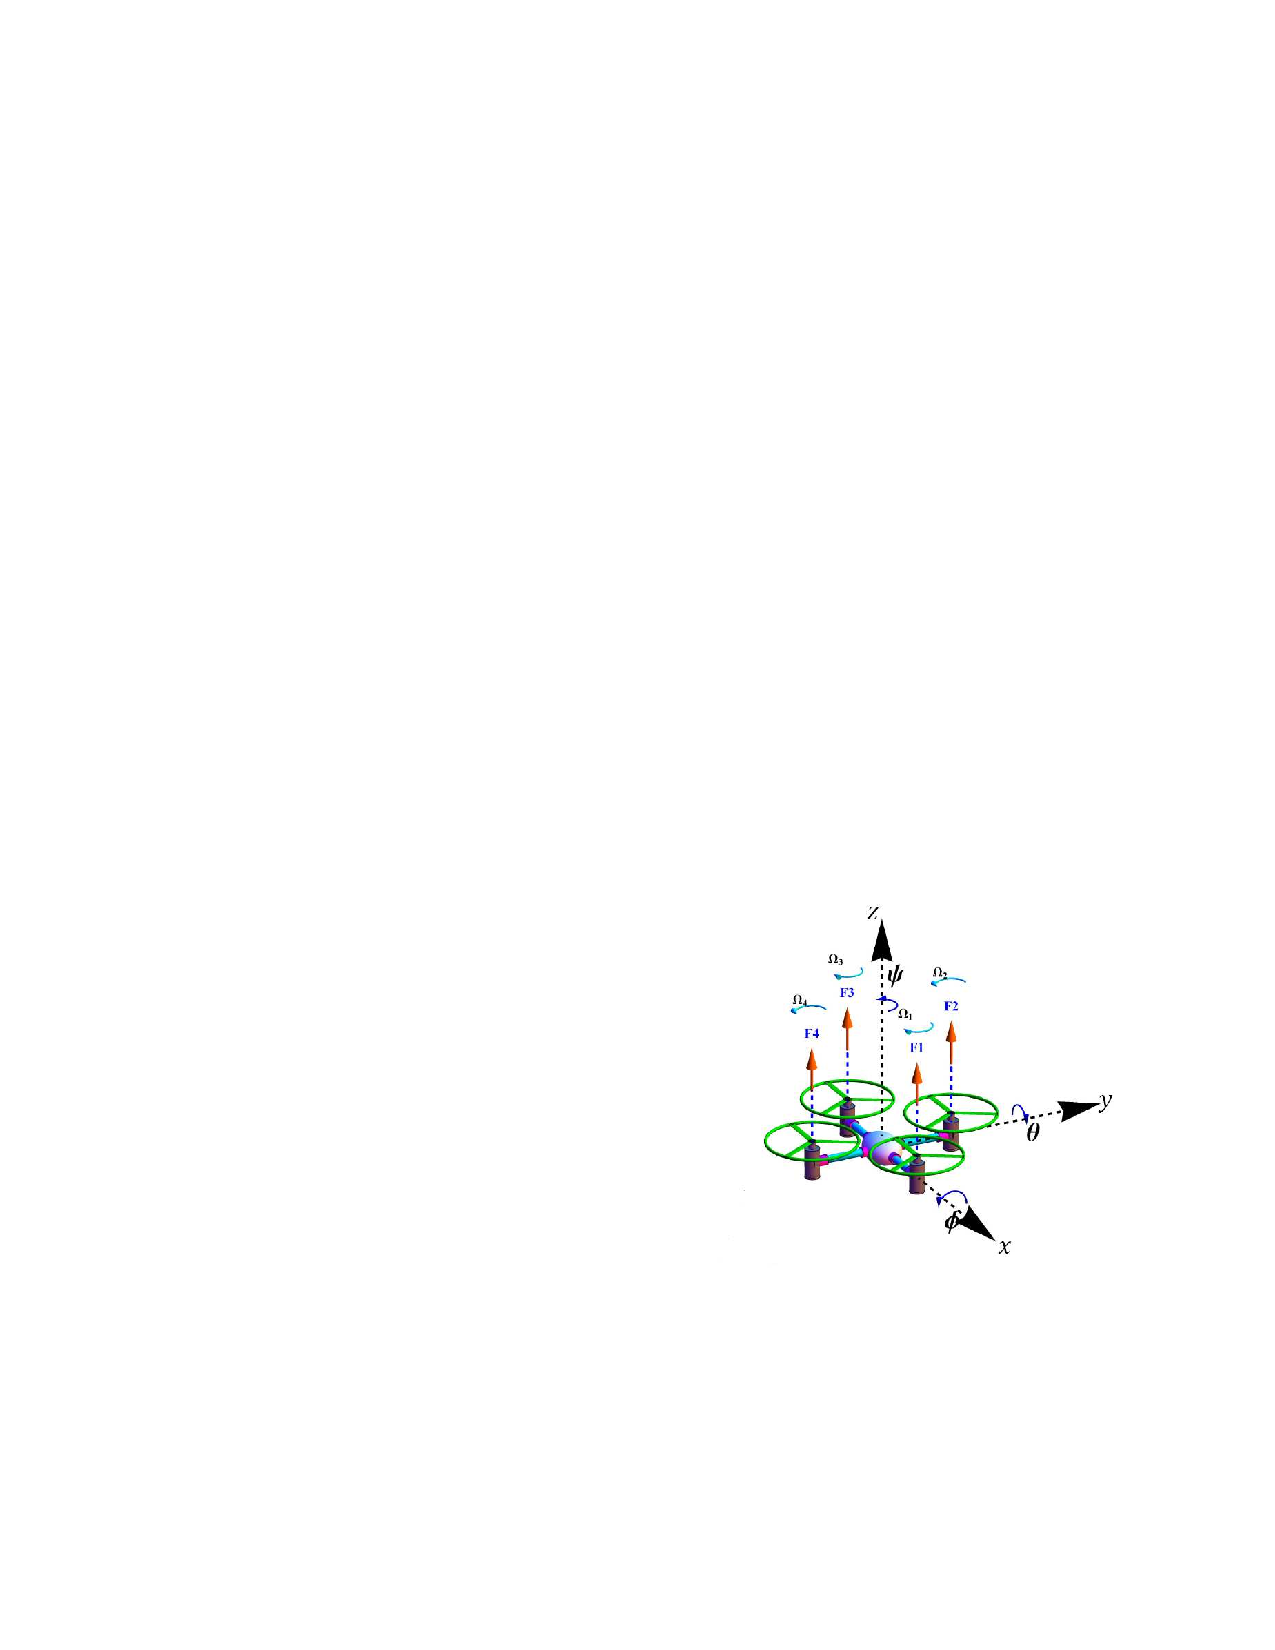
\includegraphics{images/MulticopterKraefte.pdf}
  \caption{Schubkräfte der Motoren}
  \label{fig:schubkraefte}
\end{figure} 

Im Folgendem entspricht \\
\begin{tabular}[t]{|l|l|}
  \hline
  $m_{ges}$ & Gesamtmasse des Multikopters \\ 
  $g$     & Gewichtskraft \\
  $I_{ges}$ & Gesamter Trägheitsmoment des Quadrocopters im System $B_1$\\
  ${_{M_i} I_{M_i}}$ & Trägheitmoment der Motoren im $i$-ten Motorsystem\\
  ${_{1}v_{1}}$ & Translatorische Geschwindigkeit des Körpers $B_1$ relativ zum $B_0$ System im $B_1$ System \\
  ${_{1}\omega_{1}}$ & Rotationsgeschwindigkeit des Körpers $B_1$ relativ zum $B_0$ System im $B_1$ System \\
  ${_{M_i} {\omega}_{1, M_i}}$ & Analog wie ${_{1}\omega_{1}}$\\
  ${_{M_i} {r}_{1, M_i}}$ & Abstand zwischen $B_{1}$ und $B_{2}$ mit Länge $d$ \\
  $A_{0,1}$ & Rotationsmatrix von Körper $B_1$ ins $B_0$ System \\
  $A_{1,M_i}$ & Rotationsmatrix von Körper $B_i$ ins $B_1$ System\\
  \hline
\end{tabular}\\

Mit der nicht eingezeichneten Gewichtskraft führt dies zu folgendem Kräftegleichgewicht im KOS($B_0$).
\begin{align}
    \frac{d}{dt} F_{ges} &= m_{ges} \cdot \frac{d}{dt} {_{1}v_{1}} = m_{ges} \frac{d_1}{dt} {_{1}v_{1}} + {_{1}\omega_{1}} \times m_{ges} {_{1}v_{1}} \\
    &=  {_{1}F_g} + \sum_{i = 1}^{4}{_{1}F_{i}}  \\\notag
    &= m_{ges} A_{1, 0} \cdot \begin{pmatrix} 0 \\ 0 \\ -g \end{pmatrix} + \sum_{i = 1}^4 {A_{1, M_i} \cdot _{M_i}F_{M_i}} \\
    &= m_{ges} A_{1, 0} \cdot \begin{pmatrix} 0 \\ 0 \\ -g \end{pmatrix} + \sum_{i = 1}^4 {\begin{pmatrix} 0 \\ 0 \\ F_i \end{pmatrix}}
\end{align}

Die Rotationsmatrix $A_{1, M_i}$ ändert sich je nach Konfiguration des Multikopters. Die Abbildung \ref{fig:Konfigurationen} zeigt die behandelten Konfigurationen.
\begin{figure}[ht]
  \centering
  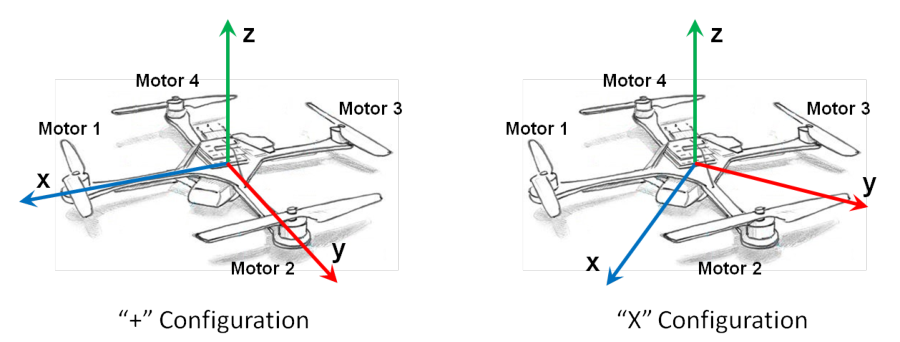
\includegraphics{images/Konfigurationen.pdf}
  \caption{Konfigurationen}
  \label{fig:Konfigurationen}
\end{figure}
Je nach Konfiguration entstehen folgende Konfigurationsmatrizen:\\\\
Für die ``+'' - Konfiguration werden folgende Matrizen verwendet:
\[
  A_{1, M_1} = \begin{pmatrix} 1 & 0 & 0 \\ 0 & 1 & 0 \\ 0 & 0 & 1 \end{pmatrix}
  A_{1, M_2} = \begin{pmatrix} 0 & -1 & 0 \\ 1 & 0 & 0 \\ 0 & 0 & 1 \end{pmatrix}
  A_{1, M_3} = \begin{pmatrix} -1 & 0 & 0 \\ 0 & -1 & 0 \\ 0 & 0 & 1 \end{pmatrix} 
  A_{1, M_4} = \begin{pmatrix} 0 & 1 & 0 \\ -1 & 0 & 0 \\ 0 & 0 & 1 \end{pmatrix}
\] \label{sec:konfg_matrix}
Für die ``x'' - Konfiguration werden folgende Matrizen verwendet:
\[
  A_{1, M_1} = \begin{pmatrix} \frac{\sqrt{2}}{2} & \frac{\sqrt{2}}{2} & 0 \\ \frac{-\sqrt{2}}{2} & \frac{\sqrt{2}}{2} & 0 \\ 0 & 0 & 1 \end{pmatrix} \hspace{0.5em}
  A_{1, M_2} = \begin{pmatrix} \frac{\sqrt{2}}{2} & -\frac{\sqrt{2}}{2} & 0 \\ \frac{\sqrt{2}}{2} & \frac{\sqrt{2}}{2} & 0 \\ 0 & 0 & 1 \end{pmatrix}
\]
\[
  A_{1, M_3} = \begin{pmatrix} -\frac{\sqrt{2}}{2} & -\frac{\sqrt{2}}{2} & 0 \\ \frac{\sqrt{2}}{2} & -\frac{\sqrt{2}}{2} & 0 \\ 0 & 0 & 1 \end{pmatrix} \hspace{0.5em}
  A_{1, M_4} = \begin{pmatrix} -\frac{\sqrt{2}}{2} & \frac{\sqrt{2}}{2} & 0 \\ -\frac{\sqrt{2}}{2} & -\frac{\sqrt{2}}{2} & 0 \\ 0 & 0 & 1 \end{pmatrix}
\]
\\
Für das Kräftegleichgewicht sind die Matrizen nicht relevant, jedoch für den folgenden Drallsatz im körperfesten System $B_1$. %Zuvor wird der Drallsatz im körperfesten System der Motoren betrachtet. Dort wirkt dem Drehmoment der Motoren $M_i$ ein Reaktionsdrehmoment  $\tau_i$ entgegen:
Zuvor wird ein fest montierter Motor betrachtet mit dem Drehmoment $M$. Diesem wirkt ein Strömungswiderstand $\tau_{drag}$ entgegen und es gilt: 
\begin{align}
{I_{rot}} \cdot \dot{\omega}  = M - \tau_{drag} 
\end{align}

Dabei ist $I_{rot}$ das Trägheitsmoment des Rotors entlang seiner z-Achse. Der Strömungswiderstand ist in der Literatur \cite{LQR2013} folgenderweise definiert als:
\begin{align}
    \tau_{drag} = \frac{1}{2} \rho A_r v^2
\end{align}
$\rho$ ist die Luftdichte, $A_r$ die Fläche, die der Rotor bei der Umdrehung überschreitet und $v$ ist die Geschwindigkeit relativ zur Luft. Näherungsweise gilt: $\omega \approx \frac{v}{r}$ und es folgt:
\begin{align}
    \tau_{drag} \approx k_{drag} \omega^2
\end{align}
Die Konstante $k_{drag} > 0$ ist abhängig von der Luftdichte, dem Radius, der Form des Propellers und anderen Faktoren. Für quasistationär Manöver ist $\omega$ konstant und es gilt: 
\begin{align}\label{gl:MDrag}
    M = \tau_{drag} \approx k_{drag} \omega^2 
\end{align}

Neben dem Drehmoment der Rotoren wird auch deren Schubkraft benötigt. Die Literatur \cite{LQR2013} gibt folgende Formel an:
\begin{align}
    F_s = C_T \rho A_r r^2 \omega^2 
\end{align}
$C_T$ ist der Schubkoeffizient für einen speziellen Rotor, $\rho, A_r$ ist wie oben, die Dichte der Luft bzw. die Fläche die, der Rotor bei der Umdrehung überschreitet. Analog führen wir einen vereinfachten Koeffizienten ein:

\begin{align}\label{gl:schub}
    F_s \approx k_{T} \omega^2 
\end{align}

Im Folgenden wird die Annahme getroffen, dass sich der Quadrocopter in einem quasistationären Zustand befindet, d.h. $\omega = const$\\

Dann gilt für Drallsatz im $B_{M_i}$ System: 
\begin{align}
    {_{M_i} I_{M_i}} {_{M_i} \dot{\omega}_{M_i}} &+ {_{M_i} {\omega}_{1}} \times {_{M_i} I_{M_i}} {_{M_i} {\omega}_{M_i}} = {_{M_i} I_{M_i}} \left({_{M_i} \dot{\omega}_{1}} + {_{M_i} \dot{\omega}_{1, M_i}}\right) \\
    &+ {_{M_i} {\omega}_{1}} \times {_{M_i} I_{M_i}} \left({_{M_i} {\omega}_{1}} + {_{M_i} {\omega}_{1, M_i}} \right) \underbrace{\approx}_{{_{M_i} {\omega}_{1}} << {_{M_i} {\omega}_{1, M_i}}} {_{M_i} I_{M_i}} {_{M_i} \dot{\omega}_{1,M_i}} \\
    &+ {_{M_i} {\omega}_{1}} \times {_{M_i} I_{M_i}} {_{M_i} {\omega}_{1, M_i}} = M_i - {_{M_i} \tau_{M_i}}
\end{align}
Zudem folgt wegen Stationärflug:
\begin{align}
    \underbrace{{_{M_i} I_{M_i}} {_{M_i} \dot{\omega}_{1, M_i}}}_{=0\text{, da }\omega =\text{ const}} + {_{M_i} {\omega}_{1}} \times {_{M_i} I_{M_i}} {_{M_i} {\omega}_{1, M_i}} = {_{M_i} {\omega}_{1}} \times {_{M_i} I_{M_i}} {_{M_i} {\omega}_{1, M_i}} =  M_i - {_{M_i} \tau_{M_i}} 
\end{align}
Dem Drehmoment der Motoren $M_i$ wird ein Gegendrehmoment ${_{M_i}\tau_{M_i}}$ entgegen gesetzt. Dieses Drehmoment findet sich auch wieder im Drallsatz des System $B_{1}$

\begin{align}
    I_{ges} {_{1} \dot{\omega}_{1}} + {_{1} {\omega}_{1}} \times I_{ges} {_{1} {\omega}_{1}} = (\tau_{R} + \tau_{P}) -\sum_{i = 1}^{4} {_{1} \tau_{M_i}} 
\end{align}

Die Drehmomente $\tau_R$ und $\tau_P$ ergeben sich aus den Roll $f_2 + f_4$ - und Nickkräfte $f_1 + f_3$: 
\begin{align}
    \tau_R = A_{1, M_1} {_{M_1}r_{1, M_1}} \times F_1  +  A_{1, M_3} {_{M_3}r_{1, M_3}} \times F_3 \\
    \tau_P = A_{1, M_2} {_{M_2}r_{1, M_2}} \times F_2  +  A_{1, M_4} {_{M_4}r_{1, M_4}} \times F_4
\end{align}

Das Gegendrehmoment ${_{M_i} \tau_{M_i}}$ ist äquivalent mit ${_{1} \tau_{M_i}}$, da der Übergang von System $B_{M_i}$ ins $B_{1}$ System eine Rotation um die z-Achse darstellt und ${{M_i} \tau_{M_i}}$ nur eine z-Komponente besitzt. Somit folgt für den ganzen Drallsatz:

\begin{align}
    I_{ges} {_{1} \dot{\omega}_{1}} + {_{1} {\omega}_{1}} \times I_{ges} {_{1} {\omega}_{1}} &+ \sum_{i=1}^{4}{{_{1} {\omega}_{1}} \times {_{M_i} I_{M_i}} {_{M_i} {\omega}_{1, M_i}}} \\
    &= -\sum_{i = 1}^{4}{M_i} + (\tau_{R} + \tau_{P})
\end{align}
$I_{ges}$ stellt das Trägheitsmoment des Körpers 1, d.h. des Quadrokopters ohne rotierende Objekte, dar. ${_{M_i} I_{M_i}}$ hingegen ist das Trägheitsmoment, eines einzelnen Rotors $i$. Bei Brushlesh Motoren ist es so, das sich die ``Wand'' mitdreht. Dies muss die Kalkulation des Trägheitsmomentes ${_{M_i} I_{M_i}}$ mit einbezogen werden.\\
Da ${_{M_i} {\omega}_{1, M_i}}$ nur eine z - Komponente besitzt mit $\omega_{M_i}$, lässt sich Gleichung folgendermassen vereinfachen.
\begin{align}
    I_{ges} {_{1} \dot{\omega}_{1}} + {_{1} {\omega}_{1}} \times I_{ges} {_{1} {\omega}_{1}} &+ \sum_{i=1}^{4}{({_{1}{\omega}_{1}} \times e_z) \cdot I_{M} \omega_{M_i} } \\
    &= \begin{bmatrix} 0 \\ 0 \\ -\sum_{i = 1}^{4}{M_i} \end{bmatrix} + (\tau_{R} + \tau_{P})
\end{align}\\\\
Für die + Konfiguration entsteht mit \ref{sec:konfg_matrix} nun folgendes Modell:
\begin{align}
    {_{0}\dot{r}_{1}} &= A_{0, 1} {_{1}v_{1}} \\
    m_{ges} \frac{d_1}{dt} {_{1}v_{1}} &+ {_{1}\omega_{1}} \times m_{ges} {_{1}v_{1}} = m_{ges} A_{1, 0} \cdot \begin{pmatrix} 0 \\ 0 \\ -g \end{pmatrix} + \sum_{i = 1}^4 {\begin{pmatrix} 0 \\ 0 \\ F_i \end{pmatrix}} \\
    {{\dot{A}_{0, 1}}} &= {A_{0, 1}} \tilde{_{1} {\omega}_{1}}\\
    I_{ges} {_{1} \dot{\omega}_{1}} &+ {_{1} {\omega}_{1}} \times I_{ges} {_{1} {\omega}_{1}} + \sum_{i=1}^{4}{({_{1}{\omega}_{1}} \times e_z) \cdot I_{M} {_{M_i}\omega_{M_i}} } \\
    &= \begin{bmatrix} 0 \\ 0 \\ -\sum_{i = 1}^{4}{M_i} \end{bmatrix} + (\tau_{R} + \tau_{P}) = \begin{bmatrix} d(F_2 - F_4) \\ d(F_3 - F_1) \\ -\sum_{i = 1}^{4}{M_i} \end{bmatrix}
\end{align}

Mit \ref{gl:MDrag} und \ref{gl:schub}
\begin{align}
    {_{0}\dot{r}_{1}} &= A_{0, 1} {_{1}v_{1}} \\
    m_{ges} \frac{d_1}{dt} {_{1}v_{1}} &+ {_{1}\omega_{1}} \times m_{ges} {_{1}v_{1}} = m_{ges} A_{1, 0} \cdot \begin{pmatrix} 0 \\ 0 \\ -g \end{pmatrix} + {\begin{pmatrix} 0 \\ 0 \\ \sum_{i = 1}^4 k_{T} {_{M_i}\omega^2_{1, M_i}} \end{pmatrix}} \\
    {{\dot{A}_{0, 1}}} &= {A_{0, 1}} \tilde{_{1} {\omega}_{1}}\\
    I_{ges} {_{1} \dot{\omega}_{1}} &+ {_{1} {\omega}_{1}} \times I_{ges} {_{1} {\omega}_{1}} + \sum_{i=1}^{4}{({_{1}{\omega}_{1}} \times e_z) \cdot I_{M} {_{M_i}\omega_{M_i}} } \\
    &= \begin{bmatrix} 0              & d \cdot k_{T} & 0             & -d \cdot k_{T} \\ 
                       -d \cdot k_{T} & 0             & d \cdot k_{T} & 0  \\
                       -k_{drag}      & k_{drag}      & -k_{drag}    & k_{drag}
       \end{bmatrix}
    \cdot 
    \begin{bmatrix}
      {_{M_1} {\omega}^2_{M_1}} \\
      {_{M_2} {\omega}^2_{M_2}}\\
      {_{M_3} {\omega}^2_{M_3}}\\
      {_{M_4} {\omega}^2_{M_4}}
    \end{bmatrix}
\end{align}
\subsubsection{Quaternionen}\label{subsub:Quaternionen}
Statt mit Eulerwinkel wird die Rotationsmatrix $A_{0, 1}$, welche die Vektoren vom Bezugssystem ins Körpersystem transformiert, mit Hilfe von Quaternionen berechnet. Dies bringt den Vorteil das kritische Punkte, also Punkte dessen Zuordnung nicht lokal umkehrbar, nicht spezifisch betrachtet werden müssen. Es bringt aber den Nachteil mit sich, dass für eine sinnvolle Auswertung der Quaternionen, diese normiert sein müssen.
\\
Die Rotationsmatrix für Quaternionen lautet: 
\begin{align}
A_{0, 1} := R_{0, 1}(q) = \left[ \begin{matrix} 1-2(q_2^2 + q_3^2) &
-2q_0q_3+2q_1q_2 &
2q_0q_2+2q_1q_3 \\
2q_0q_3+2q_1q_2 &
1-2(q_1^2 + q_3^2) &
-2q_0q_1+2q_2q_3 \\
-2q_0q_2+2q_1q_3 &
2q_0q_1+2q_2q_3 &
1-2(q_1^2 + q_2^2)
\end{matrix}
\right]
\end{align}
nach \cite{Richter2009}.\\ 
Die Zeitableitung der Quaternionen $q$ lässt nach \cite{Chou1992}, wie folgt berechnen: $\dot q = \frac{1}{2} q \otimes \begin{bmatrix} 0 \\ \omega \end{bmatrix}$. \\
\\
Somit folgt für das dynamische System des Quadrocoptors in der ``+''- Konfiguration:
\begin{align}
    {_{0}\dot{r}_{1}} &= R_{0, 1}(q) {_{1}v_{1}} \\
    \dot q &= \frac{1}{2} q \otimes \begin{bmatrix} 0 \\ \omega \end{bmatrix} \\
    m_{ges} \frac{d_1}{dt} {_{1}v_{1}} &+ {_{1}\omega_{1}} \times m_{ges} {_{1}v_{1}} = R(q)^T \begin{pmatrix} 0 \\ 0 \\ -m_{ges} \cdot g \end{pmatrix} + {\begin{pmatrix} 0 \\ 0 \\ \sum_{i = 1}^4 k_{T} {_{M_i}\omega^2_{1, M_i}} \end{pmatrix}} \\
    I_{ges} {_{1} \dot{\omega}_{1}} &+ {_{1} {\omega}_{1}} \times I_{ges} {_{1} {\omega}_{1}} + \sum_{i=1}^{4}{({_{1}{\omega}_{1}} \times e_z) \cdot I_{M} {_{M_i}\omega_{M_i}} } \\
    &= \begin{bmatrix} 0              & d \cdot k_{T} & 0             & -d \cdot k_{T} \\ 
                       -d \cdot k_{T} & 0             & d \cdot k_{T} & 0  \\
                       -k_{drag}      & k_{drag}      & -k_{drag}    & k_{drag}
       \end{bmatrix}
    \cdot 
    \begin{bmatrix}
      {_{M_1} {\omega}^2_{M_1}} \\
      {_{M_2} {\omega}^2_{M_2}}\\
      {_{M_3} {\omega}^2_{M_3}}\\
      {_{M_4} {\omega}^2_{M_4}}
    \end{bmatrix}
\end{align}

Da die Schrittweite des ODE - Lösers in unserem Lösungsansatz deutlich kleiner als 1 ist, wird die Normierung der Quaternionen mit Hilfe des Korrekturterms 
\begin{align}
  \begin{matrix}
    q_1 = ... + \lambda \dot q_1\\
    q_2 = ... + \lambda \dot q_2\\
    q_3 = ... + \lambda \dot q_3\\
    q_4 = ... + \lambda \dot q_4\\
    \text{mit } \lambda = 1- (q_1^2 + q_2^2 + q_3^2 +q_4^2)
  \end{matrix}
\end{align} gelöst \cite{Cooke1992}.

Für das Projekt wurde nun $\dot{x} = f(x, u) \in \R^{13}$ wie folgt gewählt:
\begin{align}\label{gl:ODE}
  f(x, u) &:= 
  \begin{bmatrix}
    R_{0, 1}(q) {_{1}v_{1}} \\
    \frac{1}{2} q \otimes \begin{bmatrix} 0 \\ \omega \end{bmatrix} \\
    M^{-1} (T - \Theta)
  \end{bmatrix} \\
  \text{mit } 
  T &:= \begin{bmatrix} 0\\ 0\\ -k_T \cdot \sum_{i=0}^{4}  {_{M_i} {\omega}^2_{M_i}}^2 \\ 
   K \cdot \begin{bmatrix} {_{M_1} {\omega}^2_{M_1}}^2 \\ {_{M_2} {\omega}^2_{M_2}} \\ {_{M_3} {\omega}^2_{M_3}} \\ {_{M_4} {\omega}^2_{M_4}} \end{bmatrix} +  \begin{bmatrix} 0 \\ 0 \\ 1\end{bmatrix} \times {_{1}\omega_{1}} \cdot I_M \cdot ({_{M_1} {\omega}^2_{M_1}} - {_{M_2} {\omega}^2_{M_2}} + {_{M_3} {\omega}^2_{M_3}} - {_{M_4} {\omega}^2_{M_4}})
  \end{bmatrix}
  \text{, } \\
  \Theta &:= \begin{bmatrix} m_{ges} \cdot {_{1}\omega_{1}} \times {_{1}v_{1}} + R(q)^T \cdot \begin{bmatrix} 0 \\ 0 \\ g \end{bmatrix} 
  \end{bmatrix} \text{ und } \\
  M &:= diag(m, m, m, I_{ges_1}, I_{ges_2}, I_{ges_3}) \text{ sowie für }\\
  x &:=[r_1, r_2, r_3, q_1, q_2, q_3, q_4, v_1, v_2, v_3, \omega_1, \omega_2, \omega_3 ] \text{ und } \\
  u &:=[{_{M_1} {\omega}_{M_1}}, {_{M_2} {\omega}_{M_2}}, {_{M_3} {\omega}_{M_3}}, {_{M_4} {\omega}_{M_4}}]\\
  K&:= \begin{bmatrix} 0              & d \cdot k_{T} & 0             & -d \cdot k_{T} \\ 
                       -d \cdot k_{T} & 0             & d \cdot k_{T} & 0  \\
                       -k_{drag}      & k_{drag}      & -k_{drag}    & k_{drag}
       \end{bmatrix}
\end{align}






% -*- root: ../main.tex -*-
\subsection{Sensitivitäten}
Das Ziel ist es später das SQP - Verfahren zu lösen. Dazu benötigt man die Jacobimatrix und Hessematrix der Zustände $h(t_{x_k}, x_{k-1}, u_{k-1})$, welche durch das Lösen der ODE berechnet werden. Aber anstatt zuerst die Differentialgleichung zu lösen und dann die Lösung nach $x$ bzw. $u$ abzuleiten, leitet man zuerst die ODE nach $x$ bzw. $u$ ab und löst erst dann die Differentialgleichung. Damit das nachfolgende Vorgehen überhaupt erlaubt ist, bzw. alle Ausdrücke wohldefiniert sind, muss $x(t)$ in allen Variablen stetig differenzierbar sein, damit man den Satz von Schwarz anwenden kann.\\ 

\subsubsection{Jacobimatrix}\label{subsub:Jacobi}

Sei $x \in \mathbb{R}^{k \cdot 13}$, $u \in \mathbb{R}^{k \cdot 4}$, $f(x, u) \in \mathbb{R}^{k \cdot 13}$ wie in \ref{gl:ODE} gewählt und in $k$ Zeitpunkten diskretisiert, so ist $f \in C^{\infty}$. Dann gibt es für die ODE $\dot {x} = f(x, u)$, wegen ihrer Lipschitzstetigkeit, nach Poincare eine eindeutige Lösung $h(x, u) \in \mathbb{R}^{k \cdot 13}$ mit 
\begin{align*}
 	\dot h(x, u) = f(h(x, u), u)
\end{align*}
Man betrachte nun die Differenzialgleichung zum Zeitpunkt $k$, es folgt für die Differenzierung nach der $x_i$ Komponente
\begin{align*}
	\frac{d}{dx^k_i} \frac{d}{dt^k} h(x^k, u^k) = \frac{d}{dx^k_i} f(h(x^k, u^k), u^k) \\
\end{align*}
Da $f \in C^{\infty}$ folgt nun, dass die Ableitungen vertauscht werden können.
\begin{align*}
\frac{d}{dt^k} \frac{d}{dx^k_i} h(x^k, u^k) = \frac{d}{dx^k_i} f(h(x^k, u^k), u^k)  &= \frac{d}{dx^k} \left[f(h(x^k, u^k), u^k) \right] \cdot \frac{d}{dx^k_i}h(x^k, u^k) \\
&+ \frac{d}{du^k}\left[ f(h(x^k, u^k), u^k)  \right] \cdot \underbrace{\frac{du^k}{dx^k_i}}_{=0}
\end{align*}
mit $A^k := \frac{d}{dx^k_i} h(x^k, u^k) \in \mathbb{R}^{13 \times 13}, i = 1..13$ folgt die ODE  
\begin{align*}
\frac{d}{dt^k} A^k &= \underbrace{\frac{d}{dx^k} \left[f(h(x^k, u^k), u^k) \right]}_{\in \mathbb{R}^{13 \times 13}} \cdot A^k := a(x^k, u^k, A^k)
\end{align*}
mit der Anfangsbedingung $A_0^k = I \in \mathbb{R}^{13 \times 13} $ \\\\
Analog folgt für die Differenzierung nach der $u_i$ Komponente
\begin{align*}
\frac{d}{dt^k} \frac{d}{du^k_i} h(x^k, u^k) &= \frac{d}{dx^k} \left[f(h(x^k, u^k), u^k) \right] \cdot \frac{d}{du^k_i}h(x^k, u^k) \\
&+ \frac{d}{du^k}\left[ f(h(x^k, u^k), u^k)  \right] \cdot \frac{du^k}{du^k_i}
\end{align*}
mit $B^k := \frac{d}{du^k_i} h(x^k, u^k) \in \mathbb{R}^{13 \times 4}, i = 1..4$ folgt die ODE 
\begin{align*}
\frac{d}{dt^k} B^k &= \underbrace{\frac{d}{dx^k} \left[f(h(x^k, u^k), u^k) \right]}_{\in \mathbb{R}^{13 \times 13}} \cdot B^k \\
&+ \underbrace{
	\frac{d}{du^k}
		\left[ f(h(x^k, u^k), u^k)  \right]
		   }_
{\in \mathbb{R}^{13 \times 4}}
		   \cdot \underbrace{I^k}_{\in \mathbb{R}^{4 \times 4}} :=b(x^k, u^k, B^k)
\end{align*}
mit folgender Anfangsbedingung $B_0^k = 0 \in \mathbb{R}^{13 \times 4}$. \\
\\
Sei $\Phi_1^k, \Phi_2^k$ Lösungen für $\frac{d}{dt^k} \Phi_1^k = a(x^k, u^k, \Phi_1^k)$ und $\frac{d}{dt^k} \Phi_2^k = b(x^k, u^k, \Phi_2^k)$ Für die Jacobimatrix $J^k \in \mathbb{R}^{13 \times 17}$ von $h(t_{x_k}, x_{k-1}, u_{k-1})$ folgt aus den Lösungen $\Phi_1^k, \Phi_2^k$; $J^k =[\Phi_1^k, \Phi_2^k]$
\subsubsection{Hessematrix}
Im Verlauf des Projektes hat sich herausgestellt, dass der Aufwand für die Berechnung der Hessematrix mit dem Butzen kollidiert. Anstatt diese zu berechnen wird sie durch eine Diagonalmatrix approximiert.

% -*- root: ../main.tex -*-
\subsection{Implementierung}
Das Modell wurde zunächst mit Hilfe des Mapleskriptes ``GenerateFunktionJacobi.mw'' generiert. Dazu wurde zunächst die Funktion $f(x, u)$ sowie die Matrizen $A$ und $B$ wurden \ref{subsub:Jacobi} berechnet.  Die Matrizen $A$ und $D$ wurden durch die Umgruppierung $Bv:=[A_{1, 1}, \dotso, A_{13, 1}, A_{1, 2}, \dotso, A_{13, 2}, \dotso, A_{13, 13}]$ und $Bv:=[B_{1, 1}, \dotso B_{13, 1}, B_{1, 2}, \dotso, B_{13, 4}]$ in die Vektorform gebracht. Für das gesamte zu lösende Differentialgleichungssystem gilt nun: $[\dot{x}, \dot{Av}, \dot{Bv}]:=[f(x, u), Av, Bv] =: F \in \mathbb{R}^{234}$. Nach dem Lösen der ODE, können die Ergebnisse wieder zu Matrizen $\Phi_1, \Phi_2$ transformiert werden, um die Jacobimatrix $J:=[\Phi_1, \Phi_2]$ zu erhalten.\\
\\ 
Durch Analyse verschiedener Löser für gewöhnliche Differentialgleichungen in Matlab (ode45, ode23, ode15s, ode23s), wurde festgestellt, dass das System steif ist. Somit wird für die Lösung der ODE, die Jacobimatrix $J_F$ für $F$ benötigt, dazu wurde in MAPLE $F$ nach $x, Av, Bv$ abgeleitet. \\
\\
Abschließend wurde mit Hilfe des CodeGeneration Package von MAPLE C Code generiert und mit Hilfe der Pythonskripte ``GenerateScript.py'' und ``GenerateDyn.py'' Ersetzungen (Bsp.: Warnungen, Datentypen) durchgeführt und mit der Templatedatei ``rtopt\_gen.template'' in festgelegte Form gebracht. Die Ausgabe der Codegenerierung wird in die C - Datei ``rtopt\_gen.c'' geschrieben. Die generierten Funktionen werden durch die Wrapperfunktionen ``f'', ``jac'' in ``dyn.c'' aufgerufen. \\
\\
Zum Lösen der ODE wurden verschiedene Softwarepakete ausgetestet (Matlab, odeint, CVODE) mit verschiedenen Lösern (Matlab: ode45, ode15s, ode23s; odeint: rosenbrock4 ohne und mit cuda; CVODE: CV\_BDF, CV\_ADAMS). Als schnellster Löser/Methode hat sich die Methode CV\_ADAMS des Softwarepaketes CVODE von Alan. C. Hindmarsh herausgestellt \cite{Hindmarsh2015}. Die Methode ``integrate'' in ``solver.c'' ruft die Funktionen des Softwarepaketes auf und gibt als Ergebnis die Zustände $h(t_{x_k}, x_{k-1}, u_{k-1})$ sowie deren Jacobimatrix $J=[\Phi_1, \Phi_2]$ zurück.
\subsubsection{Parameterfindung}
Als nächster Schritt wurden realistische Parameter mit Hilfe des Softwaretools; GUI\_Modeling des Softwarepaket \href{https://github.com/dch33/Quad-Sim}{Quad-Sim} Quadrocopter gefunden:\\
\begin{tabular}[t]{|l|l|}
  \hline
  $m_{ges}$ & $\SI{1.022}{kg}$  \\ 
  $g$     & $\SI{9.81}{kg.s^{-2}}$  \\
  $I_{ges}$ & $\mathrm{diag}(0.0093886, 0.0093886, 0.018406)\, \mathrm{kg} \cdot \mathrm{m}^2$\\
  $kT$ & $\SI{1.5e-7}{N.{RPM}^{-2}}$\\
  $kQ$ & $\SI{3.0e-9}{N.m.{RPM}^{-2}}$\\
  $d$ & $\SI{0.22}{m}$\\
  $I_M$ & $\SI{4.4466e-6}{kg.m^2}$\\
  \hline
\end{tabular}\\
\begin{figure}[ht]
  \centering
  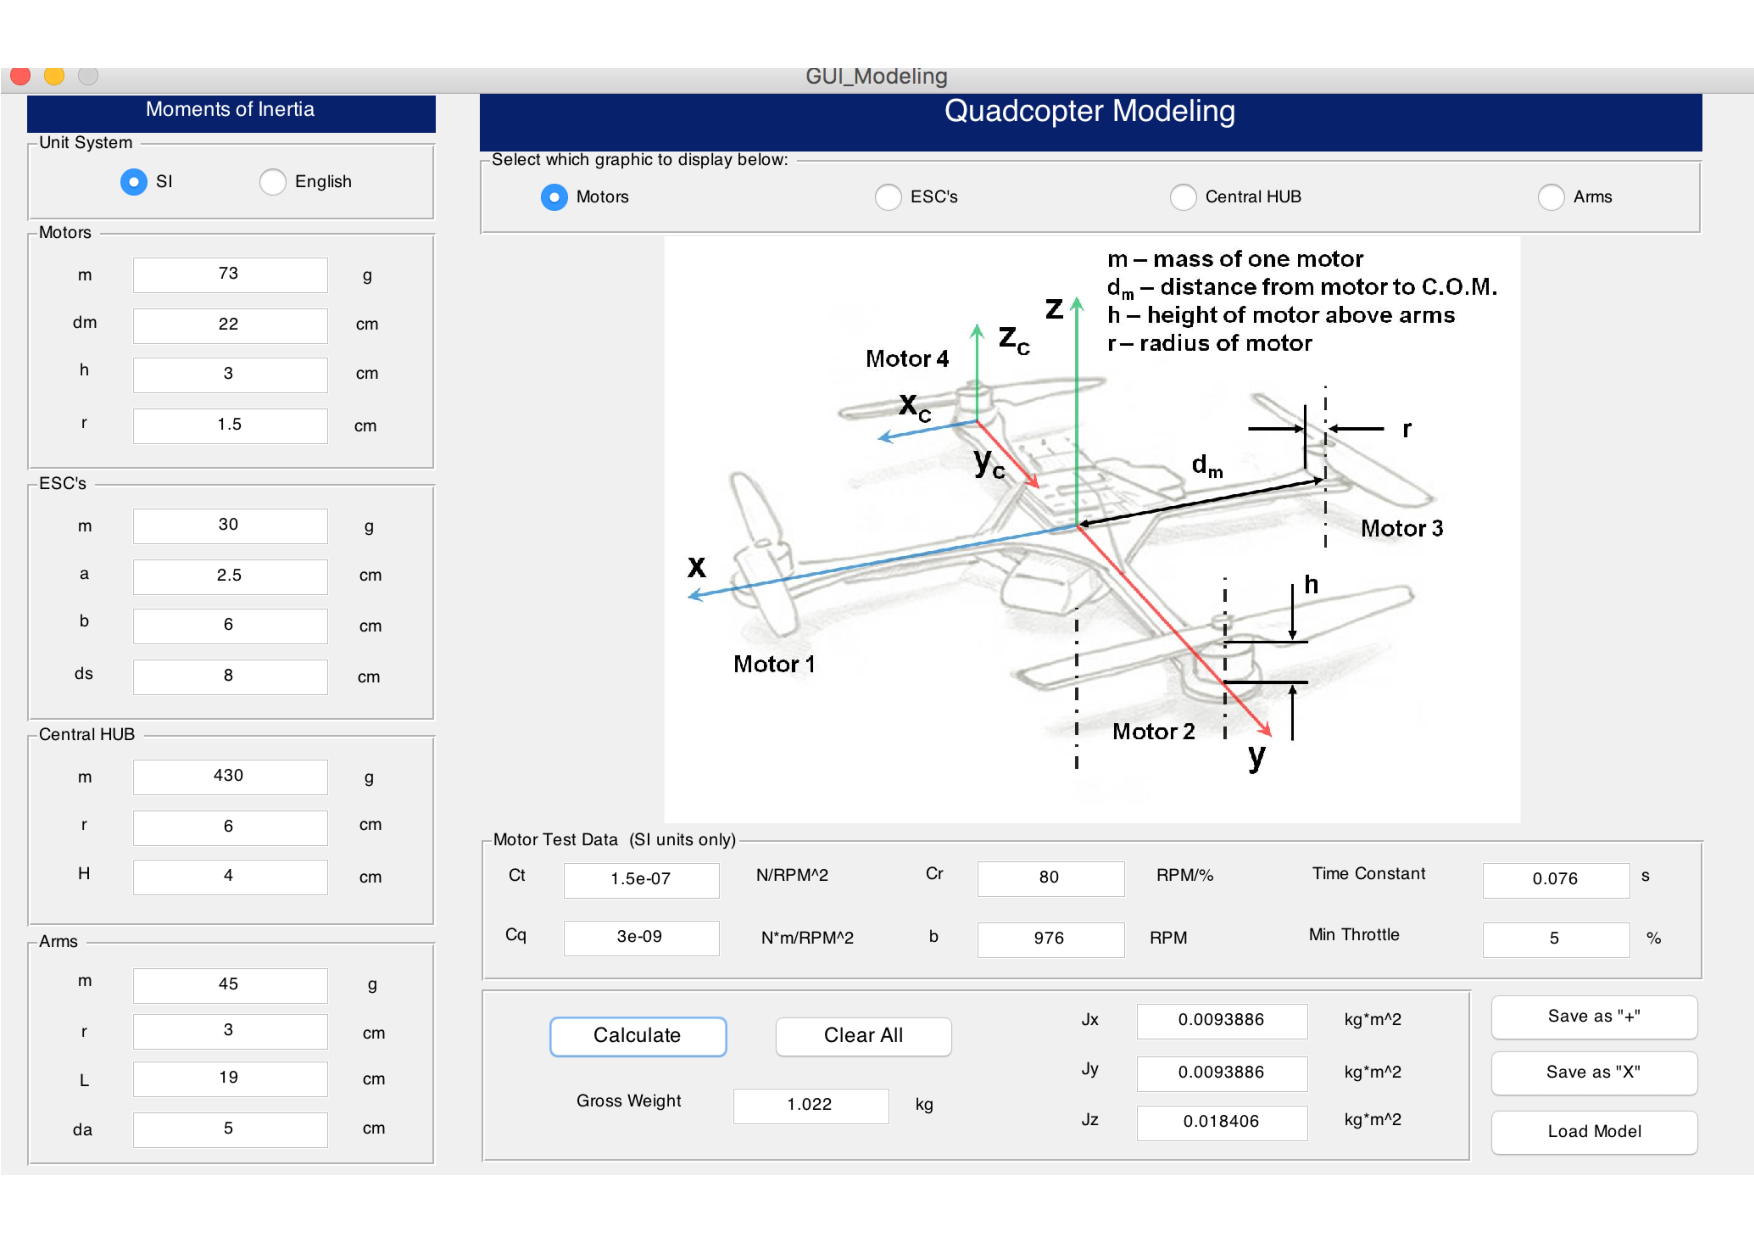
\includegraphics[width=\linewidth]{images/KonfigurationsManager.pdf}
  \caption{Konfigurationsmanager}
  \label{fig:konfigurationsmanager}
\end{figure} 
\subsubsection{Tests}
Um die Implementierung der Funktionen ``integrate'' und ``jac''zu ratifizieren wurden und die Testfunktionen ``numDiff\_nDvec'' in ``solver.c'' und ``testJac'' in ``dyn.c'' geschrieben. Für die Funktion ``integrate'' konnte nur ein qualitativer Test geschrieben werden, da die numerische Differenzierung zu ungenau für die exakte Lösung des nichtlinearen ODE System war.

% -*- root: ../main.tex -*-
\subsection{Diskretisierung}
Zu Beginn des Fluges ist der benötige Zeitraum $\Delta t$, aufgrund von der Unsicherheiten (Wind, Änderung der Flugbahn, etc.), ungekannt. Deshalb wird ein prediction horizon (Vorhersagehorizont) eingeführt. Dieser umspannt einen fixen Zeitrahmen und ist in $N$ äquidistante Punkte unterteilt. In der aktuellen Konfiguration beträgt der Abstand der einzelnen Gitterpunkte eine Sekunde. Die Zeitspanne des Horizonts darf nicht zur kurz sein, da die Berechnungen besonders bei plötzlichem Kurswechsel und starken äußeren Einflüssen zu ungenau werden. Bei zu großem Horizont benötigen die Berechnungen zu viel Zeit, so dass die Updaterate der Steuerungssignale nicht eingehalten werden kann. 
\subsection{Multiple shooting}
In den $N - 1$ Intervallen werden $N - 1$ Anfangswertprobleme gelöst mit:
\begin{align}
	\dot{s} = f(s, u) \hspace{1em} s(t_{k-1}) = s_{k-1}
\end{align}
Dabei wird der Anfangswert eines jeden Intervalls jedoch nicht fest vorgegeben, sondern als eine Variable behandelt. Da die Lösung \(h\) der Differentialgleichung auch von der Steuerung \(u\) in dem jeweiligen Intervall abhängig ist, kann man die Lösung jedes Anfangswertproblems als eine Funktion \(h=h(t,s_{i-1},q_{i-1})\) angeben. Hierbei ist also \( s_{i-1}\) der Anfangswert als Parameter, außerdem gehen wir davon aus, dass die Steuerung im Intervall \([t_{i-1},t_i]\) konstant gleich \(q(t_{i-1})=q_{i-1}\) ist.\\
Damit \(x\) eine stetige Funktion ist, soll der Anfangswert eines jeden Intervalls mit dem dem Endwert des vorigen Intervalls übereinstimmen. Dies wird als Nebenbedingung folgendermaßen in das bereits bestehenden Optimierungsproblem eingefügt:
\begin{align}
	h(t_{x_i},s_{i-1},q_{i-1}) - s_{i} = 0
	\label{equ_multiple_shooting_Nebenbedingung}
\end{align}
Diese Methode wird in der Literatur \cite{bulirsch2005} als multiple shooting method oder auch Mehrfachschießverfahren bezeichnet. Dort wird die Gleichung \ref{equ_multiple_shooting_Nebenbedingung} aber nicht mit Hilfe eines SQP - Verfahren gelöst, sondern mit Hilfe eines Newton-Verfahrens mit geschätzten Anfangswerten $x_i$, $i \in [1, N-1]$
\subsection{SQP - Methode}\label{subsec:SQP}
Mit der Diskretisierung des Optimierungsproblems und der multiple shooting method als Nebenbedingung führt dies zu dem Problem $P^k(x_k)$
\begin{align}
\min_{\begin{array}{c} s_{k},...,s_{N}\\ q_{k},...,q_{N} \end{array}} \sum_{i=k}^{N-1} j_{i}(s_{i},q_{i}) \ \  
  s.t. \ \left\lbrace \begin{array}{c}
  x_{k} - s_{k} = 0 \\
  h_i (s_i ,q_i ) - s_{i+1} = 0 \\
  g_i (s_i, q_i) \leq 0 \ \ \forall i = k, ... , N-1 \end{array} \right.
\end{align}
in jedem Zeitschritt $k$.\\
\\
Die zu den Problemen $ P^{k}(x_{k}) $ gehörenden Lagrangegleichungen lauten wie folgt:
  \begin{align}
  L^{k}(y) = \sum_{i=k}^{N-1} j_{i}(s_{i},q_{i})
  + \lambda_{k}^{T}(x_{k} - s_{k})
  + \sum_{i=k}^{N-1} \lambda_{i+1}^{T} (h_i (s_i ,q_i ) - s_{i+1})
  + \sum_{i=k}^{N-1} \mu_{i, j}^{T} (g_{i, j} (s_i, q_i))
  \end{align}
  mit $j \in \mathscr{A}(s_i, q_i):=\left\{ j: 1 \leq j \leq m; g_{i,j}(s_i, q_i)\geq 0 \right\}$

In dieser Lagrangegleichung wird $ y := (\lambda_{k},s_{k},q_{k},\mu_{k},\lambda_{k+1},s_{k+1},q_{k+1},\mu_{k+1}, ...,\lambda_{N},s_{N}) $ verwendet.
  Mit KKT-Bedingung
  \begin{align}
  \nabla_{y} L^{k}(y)  = 0
  \end{align}
  und das exakte Newton-Raphson-Verfahren
  \begin{align}
  y_{i+1} = y_i + \Delta y_i
  \end{align}
  bei dem jedes $ \Delta y_i $ die Lösung des linearen approximierten Systems
  \begin{align} 
  \nabla_{y} L^{k}(y_{i}) + J^{k}(y_{i}) \Delta y_{i} = 0
  \end{align}
  ist.\\\\
  Der von Diehl \cite{Diehl2001} vorgestellte Algorithmus verwendet das oben vorgestellte Newton-Raphson-Verfahren nicht exakt. Die zweite Ableitung $ \nabla^{2}_{y} L^{k} $, die Hesse-Matrix $ \nabla^{2}_{q,s} L^{k} $, wird ersetzt durch eine (symmetrische) Approximierung. Die Approximierung von $ \nabla^{2}_{y} L^{k}(y) $ wird im Folgenden mit $ J^{k}(y) $ bezeichnet. Ebenso wird das Newton-Type-Verfahren approximiert:
  \begin{align} 
  \nabla_{y} L^{k}(y_{i}) + J^{k}(y_{i}) \Delta y_{i} = 0
  \end{align}
  $ J^{k} $ wird auch als Karush-Kuhn-Tucker Matrix bezeichnet.\\
  \begin{align}\label{matrix:kkt}
   \nabla^{2}_{y} L^{k}(y) = 
  \begin{pmatrix}
    & -E &   &   &  &  &   &   &  &    \\
  -E& Q_k & M_k  &  & A_k^{T} &  &  &   &    &       \\
    & M_k^T & R_k & C_{i, j}^T &   B_k^{T} &  & &  &   &      \\
    &       & C_{i, j} &         &  &   & &  &    \\
    & A_k & B_k &  &   & \ddots &   & &  &    \\
    &  &  &   & \ddots & Q_{N-1} & M_{N-1} &  & A_{N-1}^{T}  &     \\
    &  &  &  &      & M_{N-1}^T  & R_{N-1} & C_{N, j}^T & B_{N-1}^{T}  &     \\
    &  &  &  &      &            & C_{N, j}  & &              &    \\
    &  &  &  &      & A_{N-1} & B_{N-1}  & &    & -E \\
    &  &  &  & &  & &  & -E & Q_{N}
  \end{pmatrix} 
\end{align}
  \\
  Mit $ A_i := \dfrac{\partial h_i}{\partial s_i} $, 
  $ B_i := \dfrac{\partial h_i}{\partial q_i} $,
  $
  \begin{pmatrix}
  Q_i & M_i \\
  M_i^{T} & R_i
  \end{pmatrix} := \nabla_{s_i,q_i}^{2}L^{i} $, \
  $C_{i, j} := \dfrac{\partial g_{i, j}}{\partial q_i}$, $j \in \mathscr{A}$
  und 
  $ Q_N := \nabla_{s_N}^{2}L^{i} $ .\\
  \\
  In der Approximierung werden $ Q_i $,$ R_i $ und $ M_i $ ersetzt durch $ Q_i^{H}(s_i,q_i,\lambda_{k+1}, \mu_{k+1}) $, $R_i^{H}(s_i,q_i,\lambda_{k+1}, \mu_{k+1}) $ und $ M_i^{H}(s_i,q_i,\lambda_{k+1}, \mu_{k+1}) $.\\
  Man betrachte  $ y = (\lambda_k, s_k,q_k, \mu_{k}, \tilde{y}) $, dass $\tilde{y}$ direkt zum nächsten Problem $ P_{k+1}(x_{k+1})$ gehört. \\
  \\
  Im Paper \cite{Diehl2002} wird erwähnt, dass diese vorteilhafte Form von $\nabla_{y}^{2} L^{k}(y) $, bzw. $ J^{k}(y) $ eine effiziente Lösung der Gleichung $ J^{k}(y)x = b $ durch die Riccati Recursion ermöglicht.\\

  \subsubsection{Approximation}\label{subsub:Approx}
  Ein wichtiger Spezialfall des Newton-Type Verfahrens ist die Constrained Gauss-Newton Methode, welche sich auf die LEAST SQUARES Form der Funktion
  \begin{align}
  \sum_{i = k}^{N-1}\frac{1}{2}\Vert l_i (s_i , q_i )\Vert_{2}^{2} +\frac{1}{2}\Vert e (s_N )\Vert_{2}^{2}
  \end{align}
  anwenden lässt. In diesem Fall lässt sich die Approximierung wie folgt berechnen:
  \begin{align}
  \begin{pmatrix}
  Q_i^{H} & M_i^{H} \\
  (M_i^{H})^{T} & R_i^{H}
  \end{pmatrix} :=
  \left( 
  \dfrac{\partial l_i (s_i,q_i)}{\partial (s_i,q_i)}
  \right) ^{T}
  \left( 
  \dfrac{\partial l_i (s_i,q_i)}{\partial (s_i,q_i)}
  \right)
  , \ \ 
  Q_N :=
  \left( 
  \dfrac{\partial e (s_N)}{\partial s_N}
  \right) ^{T}
  \left( 
  \dfrac{\partial e (s_N)}{\partial s_N}
  \right)
  \end{align}\\
  \\
  In der Praxis hat sich eine einfache Approximation von 
  $
  \begin{pmatrix}
  Q_i^{H} & M_i^{H} \\
  (M_i^{H})^{T} & R_i^{H}
  \end{pmatrix} 
  $
  durch 
$\nabla^2 l_i(s_i, q_i) + \alpha \cdot \mathrm{E}$ sehr effizient gegenüber der exakten Berechung sowie deren obrigen Approximation herausgestellt. Zudem folgt, dass die Matrix $M = 0$ ist und die Matrizen $Q$ und $R$ eine Diagonalmatrix darstellen.
\subsection{Implementierung}

Die Diskretisierung wird in der Initialisierung des Programmes in der Datei ``realtimesolver.c'' mit Funktion ``initialize\_rtsolver'' durchgeführt. Die Funktion wird im Kapitel \ref{sec:ablauf} Programmablauf  näher behandelt. 

\subsubsection{Lagrange}
Die SQP - Methode und die damit verbundene Lagrangeableitung bzw. Approximation($\nabla_{y_i} L^k(y_i)$, $J^k(y_i)$) werden in den Funktionen ``getLD'' bzw. ``getLDD'' berechnet bzw. wie in \ref{subsub:Approx} approximiert. Jene Funktionen greifen auf die Jacobi und Hessematrix der Kostenfunktion zu. Die zugehörigen Funktionen ``costD'' und ``costDD'' befinden sich in der Datei ``cost.c'' und wurden auch mit Hilfe des MAPLE - ``GenerateFunktionJacobi.mw'' und Pythonskriptes ``GenerateDyn.py'' generiert. Zudem benötigt man für die Berechnung von $\nabla_{y_i} L^k(y_i)$ und $J^k(y_i)$  die Ableitungen der Nebenbedingungen.

\subsubsection{Nebenbedingungen}
Wie in \ref{subsec:SQP} festgelegt, wird als einzige Gleichheitsnebenbedingung das Mehrfachschießverfahren gesetzt. Das Berechnen der $N-1$ Differentialgleichungen wird im Kapitel Parallelisierung \ref{parallel} erläutert.\\
\\
%Für die Ungleichungsnebenbedingungen
Damit die Steuerungssignale der Motoren nicht in einen unerlaubten Bereich fallen, wurde eine untere $u_{min}$ und eine obere $u_{max}$ Begrenzung eingeführt. Daraus ergeben sich dann acht Ungleichungsnebenbedingungen für die vier Motoren. Da man von einer Lösung nahe eines KKT - Punktes ausgehen kann, sind nur aktive Constraints interessant. Davon können aber wegen $0 \leq u_{min} < u_{max}$, nur vier Ungleichungsnebenbedingungen aktiv sein, was die Sache vereinfacht hat. Die Ungleichungsnebenbedingungen gelten aktiv, wenn gilt:
\begin{align}
  g_i(s_i, q_i) = \begin{pmatrix}
    u_{min} - q_i\\
    q_i - u_{max}
  \end{pmatrix}
  \geq 0
\end{align}
Die Implementierung der Ableitung der Ungleichungsnebenbedingungen und die Implementierung der Abfrage der aktiven Menge befinden sich in den Funktionen ``get\_ineq\_con\_at\_t\_act'' und ``checkIfActive''.
\subsubsection{Test}
Mit Hilfe der Matlab Funktion ``generateTestData'' des Matlab Projektes ``rtopt'' und der Funktion ``test\_lagrange'' in ``lagrange.c'' wurden die Ergebnisse der Funktionen ``getLD'' und ``getLDD'' validiert.





  







% -*- root: ../main.tex -*-
\section{Riccati - Rekursion}
In diesem Projekt wird die Gleichung $L^{k}(y_{i}) + J^{k}(y_{i}) \Delta y_{i} = 0$ mit Hilfe der Riccati Rekursion gelöst. Dies ist aufgrund der speziellen Form der Matrix $J^k(y^k)$ (\ref{matrix:kkt}) möglich.
Um die Übersicht zu wahren erfolgt die Herleitung der Riccati - Rekursion für die Gleichung $J^k(y^k) \delta y^k = - \nabla_{y_k} L^k(y^k)$ ohne Ungleichungsnebenbedingungen und zudem wird die Teilmatrix $M_i$ auf 0 gesetzt, d.h.
\begin{align}
    J^{k}(y) = 
  \begin{pmatrix}
    & -E &   &    &  &   &   &     \\
  -E& Q_k & 0   & A_k^{T} &  &     &    &       \\
    & 0 & R_k  &   B_k^{T} &  &   &   &      \\
    & A_k & B_k &  &   & \ddots &   &   &    \\
    &  &  &   & \ddots & Q_{N-1} & 0  & A_{N-1}^{T}  &     \\
    &  &  &  &      & 0  & R_{N-1} & B_{N-1}^{T}  &     \\
    &  &  &  &      & A_{N-1} & B_{N-1}  & &    & -E \\
    &  &  &  & &  & &  & -E & Q_{N}
  \end{pmatrix}
  \end{align}
\\
Betrachte nun
  \begin{align*}
  \begin{pmatrix}
  -E & Q_{N-1} & 0 & A_{N-1}^{T} &  \\
     & 0 & R_{N-1} & B_{N-1}^{T} &  \\
     & A_{N-1} & B_{N-1} &   & -E \\
     &   &   & -E & Q_N
  \end{pmatrix}
  \begin{pmatrix}
  \Delta \lambda_{N-1} \\
  \Delta s_{N-1} \\
  \Delta q_{N-1} \\
  \Delta \lambda_{N} \\
  \Delta s_N
  \end{pmatrix} =-
  \begin{pmatrix}
  \nabla_{s_{N-1}} L^{k}(y^{k}) \\
  \nabla_{q_{N-1}} L^{k}(y^{k}) \\
  \nabla_{\lambda_{N}} L^{k}(y^{k}) \\ 
  \nabla_{s_{N}} L^{k}(y^{k})
  \end{pmatrix}
  \end{align*}
  Zur einfacheren Schreibweise ist ab jetzt $ \nabla_{s_{N}} := -\nabla_{s_{N}} L^{k}(y^{k}) $
  \begin{align*}
  \begin{pmatrix}
   0  & A_{N-1} & B_{N-1} \\
   0  & 0  &  0 
  \end{pmatrix}
  \begin{pmatrix}
  \Delta \lambda_{N-1} \\
  \Delta s_{N-1} \\
  \Delta q_{N-1} 
  \end{pmatrix} 
  +
  \begin{pmatrix}
   0 & -E \\
   -E  &  Q_N 
  \end{pmatrix}
  \begin{pmatrix}
  \Delta \lambda_{N} \\
  \Delta s_{N} 
  \end{pmatrix} 
  = 
  \begin{pmatrix}
  \nabla_{\lambda_{N}} \\ 
  \nabla_{s_{N}} 
  \end{pmatrix}
  \end{align*}
  Für das Verfahren setzt man $ P_N = Q_N $.
  \begin{align*}
  \begin{pmatrix}
  \Delta \lambda_{N} \\
  \Delta s_{N} 
  \end{pmatrix}
  =
  \begin{pmatrix}
   0 & -E \\
   -E  &  P_N 
  \end{pmatrix}^{-1}
  \left[ 
  \begin{pmatrix}
  \nabla_{\lambda_{N}} \\ 
  \nabla_{s_{N}} 
  \end{pmatrix}
  -
  \begin{pmatrix}
   0  & A_{N-1} & B_{N-1} \\
   0  & 0  &  0 
  \end{pmatrix}
  \begin{pmatrix}
  \Delta \lambda_{N-1} \\
  \Delta s_{N-1} \\
  \Delta q_{N-1} 
  \end{pmatrix} \right] \\
  =
  \begin{pmatrix}
   -P_N & -E \\
   -E  &   
  \end{pmatrix}
  \left[ 
  \begin{pmatrix}
  \nabla_{\lambda_{N}} \\ 
  \nabla_{s_{N}} 
  \end{pmatrix}
  -
  \begin{pmatrix}
   0  & A_{N-1} & B_{N-1} \\
   0  & 0  &  0 
  \end{pmatrix}
  \begin{pmatrix}
  \Delta \lambda_{N-1} \\
  \Delta s_{N-1} \\
  \Delta q_{N-1} 
  \end{pmatrix} \right] 
  \end{align*}
  Dann werden $\Delta \lambda_{N-1}$,$\Delta s_{N-1}$ und $\Delta q_{N-1}$ gelöst.
  \begin{align*}  
  \begin{pmatrix}
  -E & Q_{N-1}+A_{N-1}^{T}P_N A_{N-1} & A_{N-1}^{T}P_N B_{N-1}  \\
   0 & B_{N-1}^{T}P_N A_{N-1} & R_{N-1}+ B_{N-1}^{T}P_N B_{N-1}
  \end{pmatrix}
  \begin{pmatrix}
  \Delta \lambda_{N-1} \\
  \Delta s_{N-1} \\
  \Delta q_{N-1} 
  \end{pmatrix}
  =
  \begin{pmatrix}
  \nabla_{s_{N-1}} \\ 
  \nabla_{q_{N-1}} 
  \end{pmatrix}
  +
  \begin{pmatrix}
  A_{N-1}^{T}P_N & A_{N-1}^{T} \\
  B_{N-1}^{T}P_N & B_{N-1}^{T}
  \end{pmatrix}
  \begin{pmatrix}
  \nabla_{\lambda_{N}} \\ 
  \nabla_{s_{N}} 
  \end{pmatrix}
  \end{align*}
  Zuerst wird $ \Delta q_{N-1}$ gelöst
  \begin{align*}
  \Delta q_{N-1} =
  (R_{N-1}+B_{N-1}^{T}P_N B_{N-1})^{-1}
  (\nabla_{q_{N-1}}+ B_{N-1}^{T}P_N \nabla_{\lambda_{N}} +
  B_{N-1}^{T}\nabla_{s_{N}} -B_{N-1}^{T}P_N A_{N-1} \Delta s_{N-1})  
  \end{align*}
  Für $\Delta \lambda_{N-1}$ und $\Delta s_{N-1}$ ergibt sich dann
  \begin{align*}
  -\Delta \lambda_{N-1} + P_{N-1}\Delta s_{N-1} = \nabla_{s_{N-1}}^{*}
  \end{align*}
  mit
  \begin{align*}
  \begin{array}{rl}
  P_{N-1} = & Q_{N-1}+A_{N-1}^{T}P_N A_{N-1} -A_{N-1}^{T}P_N B_{N-1}
  (R_{N-1}+B_{N-1}^{T}P_N B_{N-1})^{-1} B_{N-1}^{T}P_N A_{N-1} \\
  \nabla_{s_{N-1}}^{*} = & \nabla_{s_{N-1}} + A_{N-1}^{T}P_N \nabla_{\lambda_{N}} + A_{N-1}^{T}\nabla_{s_{N}} \\
   & - A_{N-1}^{T}P_N B_{N-1}(R_{N-1}+B_{N-1}^{T}P_N B_{N-1})^{-1}(\nabla_{q_{N-1}} +B_{N-1}^{T}P_N \nabla_{\lambda_{N}} +B_{N-1}^{T}\nabla_{s_{N}})
  \end{array}
  \end{align*}
  Damit ergibt sich für das anfängliche System $ J^{k}(y^{k})\Delta y^{k} = -\nabla_{y^{k}} L^{k}(y^{k})$
  \begin{align*}
  \begin{pmatrix}
    & -E &   &   &   &   &   &      \\
  -E& Q_k & 0  &  A_k^{T} &  &   &    &       \\
    & 0   & R_k & B_k^{T} &  &   &   &      \\
    & A_k & B_k &     & \ddots &   &   &    \\
    &  &  & \ddots & Q_{N-2} & 0 & A_{N-2}^{T}  &     \\
    &  &  &        &  0      & R_{N-2}  & B_{N-2}^{T}  &     \\
    &  &  &        & A_{N-2} & B_{N-2}  &     & -E \\
    &  &  &  &  &  & -E & P_{N-1}
  \end{pmatrix}
  \begin{pmatrix}
  \Delta \lambda_{k} \\
  \Delta s_{k} \\
  \Delta q_{k} \\
  \vdots \\
  \Delta \lambda_{N-1} \\
  \Delta s_{N-1} 
  \end{pmatrix} =
  \begin{pmatrix}
  \nabla_{\lambda_{k}} \\
  \nabla_{s_{k}} \\ 
  \nabla_{q_{k}} \\
  \vdots \\
  \nabla_{\lambda_{N-1}} \\
  \nabla_{s_{N-1}}^{*}
  \end{pmatrix}
  \end{align*}
  Die weiteren $P_i $ ergeben sich für $ i = k+1, ..., N-1$
  \begin{align*}
  \begin{array}{rl}
  P_{i-1} = & Q_{i-1}+A_{i-1}^{T}P_i A_{i-1} -A_{i-1}^{T}P_i B_{i-1}
  (R_{i-1}+B_{i-1}^{T}P_i B_{i-1})^{-1} B_{i-1}^{T}P_i A_{i-1} \\
  \nabla_{s_{i-1}}^{*} = & \nabla_{s_{i-1}} + A_{i-1}^{T}P_i \nabla_{\lambda_{i}} + A_{i-1}^{T}\nabla_{s_{i}}^{*} \\
   & - A_{i-1}^{T}P_i B_{i-1}(R_{i-1}+B_{i-1}^{T}P_i B_{i-1})^{-1}(\nabla_{q_{i-1}} +B_{i-1}^{T}P_i \nabla_{\lambda_{i}} +B_{i-1}^{T}\nabla_{s_{i}}^{*})
  \end{array}
  \end{align*}
  Schließlich ergibt sich
  \begin{align*}
  \begin{pmatrix}
  \Delta \lambda_{k} \\
  \Delta s_{k}
  \end{pmatrix} =
  \begin{pmatrix}
  -P_k & -E \\
  -E  & 0 
  \end{pmatrix}
  \begin{pmatrix}
  \nabla_{\lambda_{k}} \\
  \nabla_{s_{k}}^{*}
  \end{pmatrix}
  \end{align*} \\
  \\
  Bis zum jetzigen Zeitpunkt der Riccati - Rekursion wird $x_k$ das Eingabesignal (bestehend aus aktueller Position, Lage, etc.) nicht benötigt. Ist dies nun bekannt, berechne $\nabla_{\lambda_{k}}=x_k -s_k $ und 
  \begin{align*}
  \Delta q_{k} =
  (R_{k}+B_{k}^{T}P_{k+1} B_{k})^{-1}
  (\nabla_{q_{k}}+ B_{k}^{T}P_{k+1} \nabla_{\lambda_{k+1}} +
  B_{k}^{T}\nabla_{s_{k+1}}^{*} -B_{k}^{T}P_{k+1} A_{k} \Delta s_{k})  
  \end{align*}
  Sende an die Steuerungseinheiten der Motoren das Signal $u_k = q_k + \Delta q_k $ und  berechne mit der Forward Recursion die restlichen Werte von $\Delta y^{k}$
  \begin{align*}
  \begin{pmatrix}
  \Delta \lambda_{i+1} \\
  \Delta s_{i+1}
  \end{pmatrix} =
  \begin{pmatrix}
  -P_{i+1} & -E \\
  -E  & 0 
  \end{pmatrix}
  \left[ 
  \begin{pmatrix}
  \nabla_{\lambda_{i+1}} \\
  \nabla_{s_{i+1}}^{*}
  \end{pmatrix} -
  \begin{pmatrix}
  0 & A_i & B_i \\
  0 & 0 & 0 
  \end{pmatrix}
  \begin{pmatrix}
  \Delta \lambda_{i} \\
  \Delta s_{i} \\
  \Delta q_{i}
  \end{pmatrix} \right] 
  \end{align*}
  Abschließend ergibt sich $y^{k+1}$ aus $ y^{k+1} = \prod ^{k+1}(y^{k} + \Delta y^{k})$.\\
  \\
  Dieses Verfahren empfiehlt sich nicht wenn $ N $ zu groß ist.\\
  Eine Alternative wäre, für große $N$, ein fixes $n$ zu wählen und das Verfahren darauf ohne kleiner werdenden Horizont anzuwenden.

\subsection{Implementierung}
Die Implementierung des Riccatialgorithmus ist in zwei Funktionen unterteilt: Einmal die Funktion ``doStep'', welche rückwärts rekursiv, d.h. $i = N \dotso 1$ $P_{i-1}$ und $\nabla_{s_{i-1}}^{*}$ berechnet. Zum anderen die Funktion ``solveStep'' die vorwärts rekursiv die Werte $\Delta \lambda_k$, $\Delta s_k$, $\Delta q_k$ und $\Delta \mu_k$ berechnet. Wie oben erwähnt, werden bei den implementierten Algorithmus die Nebenbedingungen $\Delta \mu_k$ berücksichtigt. Da die aktiven Ungleichungsnebenbedingungen nur sehr selten auftreten und die Version ohne Constraints deutlich performanter ist wie mit, wurden zwei verschiedene Versionen des Riccatialgorithmus implementiert.\\\\
Da der Algorthmus sehr rekursiv ist, wurden wiederverwendete Ergebnisse in der Struktur ``riccati\_step\_tmp'' zwischengespeichert, um die Performance zu erhöhen.
\subsubsection{Test}
Mit Hilfe der Matlab Funktionen ``generateHesse'' und ``doTestWithHorizon2'' des Matlab Projektes ``rtopt'' in der Klasse ``Lagrange'' und der Funktion ``test\_lagrange'' in ``lagrange.c'' wurden die Ergebnisse der Funktionen ``getLD'' und ``getLDD'' validiert. 

% -*- root: ../main.tex -*-
\section{Programmablaufplan}\label{sec:ablauf}
Das Hauptprogramm ``main'' ruft die Funktion ``initialize\_rtsolver'' auf, diese führt eine Diskretisierung in $N$ äquidistante Schritten durch. Zudem allokiert sie den benötigten Speicher und initialisiert den Vektor $y_0$ mit übergebenen Werten. Ein Beispiel für Initialisierung für den Zustandsvektor liefert die Funktion ``getSteadyPoint'' in ``config.c''. Der zurückgegebene Zustandsvektor liefert für einen stationären Flug  eine Lösung des Optimierungsproblems. Nach der Initialisierung werden die Werte in der Struktur ``realtimesolver\_struct'' gespeichert und an die Hauptroutine ``fminrt'' übergeben. Diese führt den Programmablauf wie Abbildung \ref{abl:Flowchart_serial} durch. Nach erfolgreichem Ablauf wird der Speicher in ``free\_rtsolver'' wieder freigeben.

\begin{figure}[H]
\centering
\resizebox {0.7\columnwidth} {!} {
  % -*- root: ../main.tex -*-
\pagestyle{empty}
\begin{tikzpicture}[%
    >=triangle 60,              % Nice arrows; your taste may be different
    start chain=going below,    % General flow is top-to-bottom
    node distance=6mm and 60mm, % Global setup of box spacing
    every join/.style={norm},   % Default linetype for connecting boxes
    ]
% ------------------------------------------------- 
% A few box styles 
% <on chain> *and* <on grid> reduce the need for manual relative
% positioning of nodes
\tikzset{
  base/.style={draw, on chain, on grid, align=center, minimum height=4ex},
  placeholder/.style={base, white, on chain, text width=12em},
  proc/.style={base, rectangle, text width=12em},
  ode/.style={proc, rounded corners, draw=black!50, dashed},
  riccati/.style={proc, fill=blue!10},
  test/.style={base, diamond, aspect=2, text width=7em},
  term/.style={proc, rounded corners},
  % coord node style is used for placing corners of connecting lines
  coord/.style={coordinate, on chain, on grid, node distance=6mm and 25mm},
  % nmark node style is used for coordinate debugging marks
  nmark/.style={draw, cyan, circle, font={\sffamily\bfseries}},
  % -------------------------------------------------
  % Connector line styles for different parts of the diagram
  norm/.style={->, draw, lcnorm},
  free/.style={->, draw, lcfree},
  cong/.style={->, draw, lccong},
  dashedline/.style={->, draw, black!50, dashed},
  it/.style={font={\small\itshape}}
}

\node [term] (t{prepare}) {Wähle Startschätzung $y^{0} \in \mathbb{R}^{N\cdot(n_{\lambda}+n_{s}+n_{q})+ (n_{\lambda_N}+n_{s_N})}$};
\node [term, join] (t{begin}) {fminrt: Hauptroutine};
% fminrt
\node [test, join] (t1) {Im Zeitintervall? $t$};
\node [test] (t2) {Im ersten Zeitintervall?};
\node [proc, join] (p1){Prüfe, ob Ungleichungsnebenbedingungen aktiv};
\node [riccati, join] (riccati_node) {Kalkulieren der $\Delta$'s mit Riccati};
\node [proc, join] {Führe Newton-Schritt durch und Initialisiere die nächste Iteration};
\node [proc, join] {Schätze die Werte des letzten Zeitschrittes durch duplizieren der Werte des vorherigen Schrittes};
\node [proc, join]  {Speichere die geschätzten Werte};
\node [proc, join] (p4) {Erhöhe den Zeitstempel um eins};


% Bedingungen
\node [term, right=of t1] (t{ende}) {Programmende};
\node [proc, right=of t2] (p2) {Berechne Kosten};
\node [proc, join] (p3) {Berechne Gleichheitsnebenbedingungen};
\node [coord, left=of p4]  (c4)  {};
\node [coord, left=of t1]  (c1)  {};
\node [coord, left=of t{begin}] (c2){};


\path (t1.south) to node [near start, xshift=1em] {Ja} (t2);
   \draw [->,lcnorm] (t1.south) -- (t2);
\path (t1.east) to node [near start, yshift=1em] {Nein} (t{ende});
   \draw [->,lcnorm] (t1.east) -- (t{ende});
\path (t2.south) to node [near start, xshift=1em] {Ja} (p1);
   \draw [->,lcnorm] (t2.south) -- (p1);
\path (t2.east) to node [near start, yshift=1em] {Nein} (p2);
   \draw [->,lcnorm] (t2.east) -- (p2);
\draw let \p{coor} = ($ (p3.south) - (p1.east) $)
        in 
          [->,lcnorm] (p3.south) -- ++(0, -\y{coor}) -- (p1.east);
\draw [->,lcnorm] (p4.west) -- ([xshift=-1.25em]c4) -- ([xshift=-1.25em]c1) -- ([xshift=-1.25em]c2) -- (t{begin}.west);

% calculateSolution: Kalkulieren der Deltas mit Riccati
\node [placeholder, right=of t{begin}] (ph1) {};
\node [term, right=of ph1](t{begin1}) {Kalkulieren der $\Delta$'s mit Riccati};
\node [proc, join] {Setze Horizontindex auf $N$};
\node [test, join] (p{horizon}) {Ist Horizontindex $i \ge 1$?};
\node [proc] (p{Riccati}) {Löse ersten Riccarti - Schritt};
\node [proc, join] {Berechne aktuelle Steuerungssignale und führe sie aus};
\node [proc, join] (p{savRiccati}){Speichere das Ergebnis des ersten Riccati - Schritts};
%\node [proc, join] {Löse die restlichen Riccati - Schritte}
\node [test, join] (p{horizon2}) {Ist Horizontindex $\ge 2$?};
\node [term] (t{Back}) {Zurück};

\node [placeholder, right=of t{begin1}](phi2){};
\node [proc, right=of p{horizon}] (p{LagrangeAbl}) {Berechne $\nabla_{y_i} L^{i}(y)$};
\node [proc, join] (p{LagrangeJ}) {Berechne $J^{i}(y_i)$};
\node [proc, join] {Führe Riccati - Schritt aus};
\node [proc, join] (p{RiccatiStep}) {Verringere den Horizontindex um eins};

\path[rounded corners, draw=black!50, dashed]
            ([xshift=-0.75em, yshift=0.75em]p{LagrangeAbl}.north west) rectangle ([xshift=0.75em, yshift=-0.75em]p{LagrangeJ}.south east);

\node [ode, fill=red!50, above=of p{LagrangeAbl}, yshift=4em](p{ode}){Löse das Anfangswertproblem des Quadrocopter Modell für den $i$ - ten Schritt};

\node [proc, right=of p{horizon2}] (p{Riccatii}) {Löse für den Horizontindex den Riccati - Schritt};
\node [proc, join] (p{Riccatii1}) {Erhöhe den Horizontindex um eins};

\node [coord, right=of phi2] (c{begin1}) {};
\node [coord, right=of p{RiccatiStep}] (c{RiccatiStep}){};
\node [coord, right=of p{savRiccati}] (c{savRiccati}) {};
\node [coord, right=of p{Riccatii1}] (c{Riccatii1}) {};

\path (p{horizon}.south) to node [near start, xshift=1em] {Nein} (p{Riccati});
    \draw [->,lcnorm] (p{horizon}.south) -- (p{Riccati});

\path (p{horizon}.east) to node [near start, yshift=1em] {Ja} (p{LagrangeAbl});
    \draw [->,lcnorm] (p{horizon}.east) -- (p{LagrangeAbl});

\path (p{horizon2}.east) to node [near start, yshift=1em] {Ja} (p{Riccatii});
    \draw [->,lcnorm] (p{horizon2}.east) -- (p{Riccatii});

%\draw [->,lcnorm] (p{Riccatii}.north) -- (c{savRiccati}) -- (p{savRiccati}.east);
\draw let \p{absR} = ($ (p{savRiccati}.east) - (p{Riccatii1}.east) $)
        in 
          [->,lcnorm] (p{Riccatii1}.east) -- ([xshift=1.25em]c{Riccatii1}) -- ++(0, \y{absR}) -- (p{savRiccati}.east);

\draw let \p{absRiccati} = ($ ([xshift=-1em]t{begin1}.west) - (riccati_node.east)$)
        in
          [dashedline, <-] ([xshift=0.75em]riccati_node.east) -- ++(\x{absRiccati}-0.75em, 0);
\draw let \p{absode} = ($ ([xshift=-1em]p{ode}.south) - (p{LagrangeAbl}.north)$)
        in
          [->, dashedline] (p{ode}.south) -- ++(0, -\y{absode} + 0.75em);

\draw[->, lcnorm] (p{RiccatiStep}.east) -- ([xshift=1.25em]c{RiccatiStep}) -- ([xshift=1.25em]c{begin1}) -- (t{begin1}); 
\path (p{horizon2}.south) to node [near start, xshift=1em] {Nein} (t{Back});
    \draw [->, lcnorm] (p{horizon2}.south) -- (t{Back}); +

\path[rounded corners, draw=black!50, dashed]
            ([xshift=-0.75em, yshift=0.75em]riccati_node.north west) rectangle ([xshift=0.75em, yshift=-0.75em]riccati_node.south east);

\begin{pgfonlayer}{background}
\path[fill=blue!10,rounded corners, draw=black!50, dashed]
            ([xshift=-1em, yshift=1em]t{begin1}.north west) rectangle ([xshift=1.75em, yshift=-2em]p{Riccatii1}.south east);
\end{pgfonlayer}
\end{tikzpicture}
% ===============
  \label{abl:Flowchart_serial}
}
\caption{Serieller Programmablaufplan}
\end{figure}

\subsection{Parallelisierung}\label{parallel}
\subsubsection{Riccati}
Bei der Analyse des Riccatialgorithmus stellt man fest, dass sich der Punkt ``Kalkulieren der $\Delta$'s mit Riccati'' in der Abildung \ref{abl:Flowchart_serial}  nur sehr schwer parallelisieren lässt, da die Berechnungen von $P$, $\nabla_{s_{i-1}}^{*}$ und Co rekursiv sind, d.h. es wird zwingend einen Vorgänger bzw. Nachfolger benötigt. Einen Performancegewinn erzielt man, wie bereits erwähnt, mit dem Zwischenspeichern von wiederkehrenden Ergebnissen. Besonders die im Schritt ``Führe Riccati - Schritt aus'' erzielten Ergebnisse der lu - Zerlegung können in den Schritten ``Löse Riccati Schritt'' wiederverwendet werden. Durch die einfache Approximation der Hessematrix durch $J^i(y_i)$ ist der Aufwand zur Lösung des Gleichungssystem $\nabla_{y} L^{k}(y_{i}) + J^{k}(y_{i}) \Delta y_{i} = 0$ gegenüber dem multiple shooting in Schritt ``Paralleles Lösen der $N-1$ Anfangswertprobleme'' in der Abbildung \ref{abl:Flowchart_parallel}  vernachlässigbar.
\subsection{Multiple Shooting}
Das Lösen des Anfangswertproblems des Quadrocopter - Modells für den $i$ - ten Schritt im parallelisierten Programmablauf \ref{abl:Flowchart_parallel} wird nicht mehr durch die Schritte ``Berechne $\nabla_{y_i} L^{i}(y)$'' und ``Berechne $J^{i}(y_i)$'' aufgerufen (siehe Abbildung \ref{abl:Flowchart_serial}), sondern in dem Punkt ``Löse $N-1$ Anfangswertprobleme des Quadrocopter Modell'' ausgelagert, um eine Parallelisierung zu erreichen. Die Ergebnisse werden durch den Vektor der Struktur ``multiple\_shooting'' an die Funktionen ``getLD'' und ``getLDD'' übergeben, die für die Berechnung der Ableitung bzw. der Approximation Jacobi - bzw. Hessematrix der Lagrangefunktion zuständig sind.
\begin{figure}[H]
\centering
\resizebox {0.7\columnwidth} {!} {
  % -*- root: ../main.tex -*-
\pagestyle{empty}
\begin{tikzpicture}[%
    >=triangle 60,              % Nice arrows; your taste may be different
    start chain=going below,    % General flow is top-to-bottom
    node distance=6mm and 60mm, % Global setup of box spacing
    every join/.style={norm},   % Default linetype for connecting boxes
    ]
% ------------------------------------------------- 
% A few box styles 
% <on chain> *and* <on grid> reduce the need for manual relative
% positioning of nodes
\tikzset{
  base/.style={draw, on chain, on grid, align=center, minimum height=4ex},
  placeholder/.style={base, white, on chain, text width=12em},
  proc/.style={base, rectangle, text width=12em},
  riccati/.style={proc, fill=blue!10},
  test/.style={base, diamond, aspect=2, text width=7em},
  term/.style={proc, rounded corners},
  % coord node style is used for placing corners of connecting lines
  coord/.style={coordinate, on chain, on grid, node distance=6mm and 25mm},
  % nmark node style is used for coordinate debugging marks
  nmark/.style={draw, cyan, circle, font={\sffamily\bfseries}},
  % -------------------------------------------------
  % Connector line styles for different parts of the diagram
  norm/.style={->, draw, lcnorm},
  free/.style={->, draw, lcfree},
  cong/.style={->, draw, lccong},
  dashedline/.style={->, draw, black!50, dashed},
  it/.style={font={\small\itshape}}
}

\node [term] (t{prepare}) {Wähle Startschätzung $y^{0} \in \mathbb{R}^{N\cdot(n_{\lambda}+n_{s}+n_{q})+ (n_{\lambda_N}+n_{s_N})}$};
\node [term, join] (t{begin}) {fminrt: Hauptroutine};
% fminrt
\node [test, join] (t1) {Im Zeitintervall? $t$};
\node [test] (t2) {Im ersten Zeitintervall?};
\node [proc, join] (p1){Prüfe, ob Ungleichungsnebenbedingungen aktiv};
\node [proc, join, fill=red!50] {Löse $N-1$ Anfangswertprobleme des Quadrocopter Modells};
\node [riccati, join] (riccati_node) {Kalkulieren der $\Delta$'s mit Riccati};
\node [proc, join] {Führe Newton-Schritt durch und Initialisiere die nächste Iteration};
\node [proc, join] {Schätze die Werte des letzten Zeitschrittes durch duplizieren der Werte des vorherigen Schrittes};
\node [proc, join]  {Speichere die geschätzten Werte};
\node [proc, join] (p4) {Erhöhe den Zeitstempel um eins};


% Bedingungen
\node [term, right=of t1] (t{ende}) {Programmende};
\node [proc, right=of t2] (p2) {Berechne Kosten};
\node [proc, join] (p3) {Berechne Gleichheitsnebenbedingungen};
\node [coord, left=of p4]  (c4)  {};
\node [coord, left=of t1]  (c1)  {};
\node [coord, left=of t{begin}] (c2){};


\path (t1.south) to node [near start, xshift=1em] {Ja} (t2);
   \draw [->,lcnorm] (t1.south) -- (t2);
\path (t1.east) to node [near start, yshift=1em] {Nein} (t{ende});
   \draw [->,lcnorm] (t1.east) -- (t{ende});
\path (t2.south) to node [near start, xshift=1em] {Ja} (p1);
   \draw [->,lcnorm] (t2.south) -- (p1);
\path (t2.east) to node [near start, yshift=1em] {Nein} (p2);
   \draw [->,lcnorm] (t2.east) -- (p2);
\draw let \p{coor} = ($ (p3.south) - (p1.east) $)
        in 
          [->,lcnorm] (p3.south) -- ++(0, -\y{coor}) -- (p1.east);
\draw [->,lcnorm] (p4.west) -- ([xshift=-1.25em]c4) -- ([xshift=-1.25em]c1) -- ([xshift=-1.25em]c2) -- (t{begin}.west);

% calculateSolution: Kalkulieren der Deltas mit Riccati
\node [placeholder, right=of t{begin}] (ph1) {};
\node [term, right=of ph1](t{begin1}) {Kalkulieren der $\Delta$'s mit Riccati};
\node [proc, join] {Setze Horizontindex auf $N$};
\node [test, join] (p{horizon}) {Ist Horizontindex $i \ge 1$?};
\node [proc] (p{Riccati}) {Löse ersten Riccarti - Schritt};
\node [proc, join] {Berechne aktuelle Steuerungssignale und führe sie aus};
\node [proc, join] (p{savRiccati}){Speichere das Ergebnis des ersten Riccati - Schritts};
%\node [proc, join] {Löse die restlichen Riccati - Schritte}
\node [test, join] (p{horizon2}) {Ist Horizontindex $\ge 2$?};
\node [term] (t{Back}) {Zurück};

\node [placeholder, right=of t{begin1}](phi2){};
\node [proc, right=of p{horizon}] (p{LagrangeAbl}) {Berechne $\nabla_{y_i} L^{i}(y)$};
\node [proc, join] {Berechne $J^{i}(y_i)$};
\node [proc, join] {Führe Riccati - Schritt aus};
\node [proc, join] (p{RiccatiStep}) {Verringere den Horizontindex um eins};

\node [proc, right=of p{horizon2}] (p{Riccatii}) {Löse für den Horizontindex den Riccati - Schritt};
\node [proc, join] (p{Riccatii1}) {Erhöhe den Horizontindex um eins};

\node [coord, right=of phi2] (c{begin1}) {};
\node [coord, right=of p{RiccatiStep}] (c{RiccatiStep}){};
\node [coord, right=of p{savRiccati}] (c{savRiccati}) {};
\node [coord, right=of p{Riccatii1}] (c{Riccatii1}) {};

\path (p{horizon}.south) to node [near start, xshift=1em] {Nein} (p{Riccati});
    \draw [->,lcnorm] (p{horizon}.south) -- (p{Riccati});

\path (p{horizon}.east) to node [near start, yshift=1em] {Ja} (p{LagrangeAbl});
    \draw [->,lcnorm] (p{horizon}.east) -- (p{LagrangeAbl});

\path (p{horizon2}.east) to node [near start, yshift=1em] {Ja} (p{Riccatii});
    \draw [->,lcnorm] (p{horizon2}.east) -- (p{Riccatii});

%\draw [->,lcnorm] (p{Riccatii}.north) -- (c{savRiccati}) -- (p{savRiccati}.east);
\draw let \p{absR} = ($ (p{savRiccati}.east) - (p{Riccatii1}.east) $)
        in 
          [->,lcnorm] (p{Riccatii1}.east) -- ([xshift=1.25em]c{Riccatii1}) -- ++(0, \y{absR}) -- (p{savRiccati}.east);

\draw let \p{absRiccati} = ($ ([xshift=-1em]t{begin1}.west) - (riccati_node.east)$)
        in
          [dashedline, <-] ([xshift=0.75em]riccati_node.east) -- ++(\x{absRiccati}-0.75em, 0);

\draw[->, lcnorm] (p{RiccatiStep}.east) -- ([xshift=1.25em]c{RiccatiStep}) -- ([xshift=1.25em]c{begin1}) -- (t{begin1}); 
\path (p{horizon2}.south) to node [near start, xshift=1em] {Nein} (t{Back});
    \draw [->, lcnorm] (p{horizon2}.south) -- (t{Back}); +

\path[rounded corners, draw=black!50, dashed]
            ([xshift=-0.75em, yshift=0.75em]riccati_node.north west) rectangle ([xshift=0.75em, yshift=-0.75em]riccati_node.south east);

\begin{pgfonlayer}{background}
\path[fill=blue!10,rounded corners, draw=black!50, dashed]
            ([xshift=-1em, yshift=1em]t{begin1}.north west) rectangle ([xshift=1.75em, yshift=-2em]p{Riccatii1}.south east);
\end{pgfonlayer}
\end{tikzpicture}
% ===============
  \label{abl:Flowchart_parallel}
}
\caption{Paralleler Programmablaufplan}
\end{figure}

\subsubsection{Implementierung}
Für die Parallelisierung wurde das Message Passing Interface (MPI) gewählt, dar die Designziele die Bedürfnisse des Projektes erfüllen. Portabilität, Effizenz und Flexibilität. MPI ist kein IEEE oder ISO Standard, aber es ist tatsächlich so, dass dieses Protokoll ein Industriestandard geworden ist. Zudem unterstützen verschiedene MPI Produkte MVAPICH2, OpenMPI, CRAY, und IBM Platform MPI die Schnittstelle CUDA-aware. Dies Schnittstelle bietet eine einfache Kommunikation zwischen CUDA - GPU's und CPU, sodass dieses Projekt von reiner CPU Parallelisierung in einen Mix aus GPU und CPU Parallelisierung umgebaut werden kann. Im Nachfolgenden wird angenommen, dass die Anzahl zu lösender Differentialgleichungen $N-1$ deutlich höher ist als die Anzahl der Prozesse $P$, d.h. $P << N - 1$. Zudem existiert ein Booleanarray ``bwork'' mit $N-1$ Werten. Ist der $i$-te Eintrag wahr, so wurde bzw. wird das $i$ te Differentialgleichungssystem gelöst. Pro Prozess existiert ein temporäres ``itmp\_work'' Array mit $N-1$ ganzzahligen Elementen. Hat ein Prozess eine ODE gelöst fügt es dem ``itmp\_work'' Array in kommender Reihefolge die Ranking-Id hinzu. Dabei beginnen die Ranking-Id's mit $1$. Ist an der $k$ - ten Stelle eine Null, so ist das Array zu Ende.
Die Parallisierung hat folgenden Ablauf:


\begin{figure}[H]
\centering
\resizebox {0.7\columnwidth} {!} {
  % -*- root: ../main.tex -*-
\pagestyle{empty}
\begin{tikzpicture}[%
    >=triangle 60,              % Nice arrows; your taste may be different
    start chain=going below,    % General flow is top-to-bottom
    node distance=6mm and 60mm, % Global setup of box spacing
    every join/.style={norm},   % Default linetype for connecting boxes
    ]
% ------------------------------------------------- 
% A few box styles 
% <on chain> *and* <on grid> reduce the need for manual relative
% positioning of nodes
\tikzset{
  base/.style={draw, on chain, on grid, align=center, minimum height=4ex},
  placeholder/.style={base, white, on chain, text width=12em},
  proc/.style={base, rectangle, text width=12em},
  riccati/.style={proc, fill=blue!10},
  test/.style={base, diamond, aspect=2, text width=7em},
  term/.style={proc, rounded corners},
  % coord node style is used for placing corners of connecting lines
  coord/.style={coordinate, on chain, on grid, node distance=6mm and 25mm},
  % nmark node style is used for coordinate debugging marks
  nmark/.style={draw, cyan, circle, font={\sffamily\bfseries}},
  % -------------------------------------------------
  % Connector line styles for different parts of the diagram
  norm/.style={->, draw, lcnorm},
  free/.style={->, draw, lcfree},
  cong/.style={->, draw, lccong},
  dashedline/.style={->, draw, black!50, dashed},
  it/.style={font={\small\itshape}}
}

\node [term] {Löse $N-1$ Anfangswertprobleme des Quadrocopter Modells};
\node [test, join] (test_rank_id) {Prozess Id $=0$?};
\node [proc, join] (sende) {Sende alle Anfangsbedingungen an alle Prozesse};
\node [test, join] (bwork) {sum(bwork) $> 0$?};
\node [proc] (zufall){Wähle zufallsmäßig aus den noch nicht gelösen ODE's aus};
\node [proc, join] {Setze den Status jener ODE im ``bwork'' Array die ausgewählt wurde};
\node [proc, join] {Sende aktuelles ``bwork'' Array an alle Prozesse };
\node [proc, join] {Löse die ODE};
\node [proc, join] (save) {Speichere die Daten und setze ``itmp\_work''};

\node [coord, right=of sende] (sendeleft) {};
\node [coord, left=of save] (saveleft){};
\node [coord, left=of bwork] (bworkleft) {};

\draw [->,lcnorm] (save.west) -- ([xshift=-0.75em]saveleft) -- ([xshift=-0.75em]bworkleft) -- (bwork.west);

\path (test_rank_id.south) to node [near start, xshift=1em] {Ja} (sende);
   \draw [->,lcnorm] (test_rank_id.south) -- (sende);

\path (bwork.south) to node [near start, xshift=1em] {Ja} (zufall);
   \draw [->,lcnorm] (bwork.south) -- (zufall);


%----%
\node [proc, right=of test_rank_id] (wait){Warte auf Daten};
\path (test_rank_id.east) to node [near start, xshift=1em, yshift=1em] {Nein} (wait);
   \draw [->,lcnorm] (test_rank_id.east) -- (wait);

\draw [->,lcnorm] (wait.south) -- ([xshift=9.15em, yshift=-1em]sendeleft) -- (bwork.north);



%---%
\node [test, right=of bwork] (test_rank_id1) {Prozess Id $=0$?};
\node [proc, join] (reciv0){Empfange Lösungen von anderen Prozessen};
\node [test, join] (reciv) {Alle Lösungen empfangen?};
\node [proc] (prepare) {Bereite Daten auf};
\node [term, join] (ende){Prozedurende};

\node [coord, right =of reciv0] (recivright0) {};
\node [coord, right =of reciv] (recivright) {};
\node [coord, right =of ende] (enderight){};


\path (reciv.east) to node [near start, xshift=1em, yshift=1em] {Nein} (recivright);
   \draw [->,lcnorm] (reciv.east) -- ([xshift=1em]recivright) -- ([xshift=1em]recivright0) -- (reciv0);

\path (bwork.east) to node [near start, xshift=1em, yshift=1em] {Nein} (test_rank_id1.west);
   \draw [->,lcnorm] (bwork.east) -- (test_rank_id1.west);

\path (reciv.south) to node [near start, xshift=1em] {Ja} (prepare.north);
   \draw [->,lcnorm] (reciv.south) -- (prepare.north);

%---%
\node [proc, right=of test_rank_id1] (sendsol) {Sende Lösungen und ``itmp\_work''};

\path (test_rank_id1.east) to node [near start, xshift=1em, yshift=1em] {Nein} (sendsol.west);
   \draw [->,lcnorm] (test_rank_id1.east) -- (sendsol.west);
\draw [->,lcnorm] (sendsol.south) -- ([xshift=9.15em]enderight.north) -- (ende);

\end{tikzpicture}
  \label{abl:Flowchart_mpi}
}
\caption{MPI - Implementierung}
\end{figure}
\section{Ausblick}

Nach der Implementierung des Projektes kann als nächster Schritt das Parallelisieren mit MPI CUDA Adware durchgeführt werden. Es besteht die Möglichkeit den Code Embedding fähig zu machen. Als Plattform könnte sich die Embedding Platform Jetson TK1 eignen. Es müssten aber noch weitere Nachforschungen getätigt werden. Abschließend sollte ein passende Konfiguration für einen Quadrocopter gefunden und eine Testumgebung mit Trackingsystem aufgebaut werden. 
% -*- root: ../main.tex -*-
\begin{appendix}
\section{Anhang}
%\input{text/MAPLE/GenerateFunktionJacobi.tex}
\begin{figure}[H]
\resizebox {0.2\columnwidth} {!} {
  % -*- root: ../main.tex -*-
\tikzstyle{every node}=[draw=black,thick,anchor=west]
\tikzstyle{selected}=[draw=red,fill=red!30]
\tikzstyle{optional}=[dashed,fill=gray!50]
\begin{tikzpicture}[%
  grow via three points={one child at (0.5,-0.7) and
  two children at (0.5,-0.7) and (0.5,-1.4)},
  edge from parent path={(\tikzparentnode.south) |- (\tikzchildnode.west)}]
  \node {Project}
    child { node {Data}}
    child { node {doc}}		
    child { node {include}
      child { node {constraints.h}}
      child { node {cost.h}}
      child { node {cs.h}}
      child { node {cs\_types.h}}
      child { node {cvode\_impl.h}}
      child { node {dyn.h}}
      child { node {lagrange.h}}
      child { node {quad\_types.h}}
      child { node {realtimesolver.h}}
      child { node {riccati.h}}
      child { node {rtopt\_gen.h}}
      child { node {solver.h}}
      child { node {sys\_base.h}}
      child { node {sys\_config.h}}
      child { node {sys\_types.h}}
      child { node {util.h}}
    }
    child [missing] {}
    child [missing] {}
    child [missing] {}
    child [missing] {}
    child [missing] {}
    child [missing] {}
    child [missing] {}
    child [missing] {}
    child [missing] {}
    child [missing] {}
    child [missing] {}
    child [missing] {}
    child [missing] {}
    child [missing] {}
    child [missing] {}
    child [missing] {}
    child { node {MAPLE}
      child { node {GenerateFunctionJacobi.mw}}
      child { node {GenerateFunctionJacobi.mpl}}
    }
    child [missing] {}
    child [missing] {}
    child { node {PYTHON}
      child { node {GenerateDyn.py}}
      child { node {GenerateScript.py}}
    }
    child [missing] {}
    child [missing] {}
    child { node {src}
      child { node {alloc\_mem.c}}
      child { node {calc\_time.c}}
      child { node {config.c}}
      child { node {cost.c}}
      child { node {cs\_ext.c}}
      child { node {diff.c}}
      child { node {dyn.c}}
      child { node {gen.c}}
      child { node {lagrange.c}}
      child { node {multipleshooting.c}}
      child { node {nrm.c}}
      child { node {output.c}}
      child { node {realtimesolver.c}}
      child { node {riccati.c}}
      child { node {rtopt\_gen.c}}
      child { node {solver.c}}
    }
    child [missing] {}
    child [missing] {}
    child [missing] {}
    child [missing] {}
    child [missing] {}
    child [missing] {}
    child [missing] {}
    child [missing] {}
    child [missing] {}
    child [missing] {}
    child [missing] {}
    child [missing] {}
    child [missing] {}
    child [missing] {}
    child [missing] {}
    child [missing] {}
    child { node {template}
      child { node {rtopt\_gen.template}}
    }
    child [missing] {}
    child { node {dyn.ini}}
    child { node {init.sh}}
    child { node {Makefile}}
    child { node {rtopt.ini}}
    child { node {setup\_dyn.sh}};
\end{tikzpicture}
  \label{abl:file_tree}
}
\caption{Dateistruktur}
\end{figure}

\begin{figure}[H]
\centering
\resizebox {\columnwidth} {!} {
  % -*- root: ../main.tex -*-
\begin{tikzpicture}[->,>=stealth']

\tikzset{
    state/.style={
           rectangle,
           rounded corners,
           draw=black, very thick,
           minimum height=2em,
           inner sep=2pt,
           text centered,
           },
}
 % Position of classDyn 
 % Use previously defined 'state' as layout (see above)
 % use tabular for content to get columns/rows
 % parbox to limit width of the listing
 \node[state] (realtimesolver) 
 {\begin{tabular}{l}
  \textbf{realtimesolver}\\
  \parbox{4cm}{\begin{itemize}
  \item vec
  \item lambda
  \item activeSet 
  \item muSet
  \item ntime
  \item nhorizon
  \item data
  \end{itemize}
  }
 \end{tabular}};
  
 % STATE QuadConfig
 \node[state,
  left of=realtimesolver,
  node distance=6.5cm,
  text width=5cm] (QuadConfig) 
 {%
 \begin{tabular}{l}
  \textbf{QuadConfig}\\
  \parbox{4.8cm}{
  \begin{itemize}
  \item g Gravitation
  \item m Masse
  \item kT
  \item kQ
  \item d Abstand
  \item IM
  \item Iges
  \item u
  \item umax
  \item umin
\end{itemize}}
 \end{tabular}
 };

 \node[state,    	% layout (defined above)
  text width=4cm, 	% max text width
  right of=realtimesolver, 	% Position is to the right of classDyn
  node distance=6.5cm, 	% distance to classDyn
  anchor=center] (riccati) 	% posistion relative to the center of the 'box'
 {%
 \begin{tabular}{l} 	% content
  \textbf{riccati}\\
  \parbox{4.8cm}{
  \begin{itemize}
  \item nhorizon
  \item nbytesDeltaMu
\end{itemize}}
 \end{tabular}
 };
\node[state,      % layout (defined above)
  text width=4cm,   % max text width
  right of=riccati,  % Position is to the right of classDyn
  node distance=6.5cm,  % distance to classDyn
  anchor=center] (riccati_step)  % posistion relative to the center of the 'box'
 {%
 \begin{tabular}{l}   % content
  \textbf{riccati\_step}\\
  \parbox{4.8cm}{
  \begin{itemize}
  \item nvar
  \item naddConstr
  \item P
  \item Q
  \item M
  \item R
  \item A
  \item B
  \item D
  \item nabla\_lambda
  \item nabla\_s\_star
  \item delta\_s
  \item delta\_lambda
  \item delta\_q
  \item delta\_mu
\end{itemize}}
 \end{tabular}
 };

 \node[state,      % layout (defined above)
  text width=4cm,   % max text width
  right of=riccati_step,  % Position is to the right of classDyn
  node distance=6.5cm,  % distance to classDyn
  anchor=center] (riccati_step_tmp)  % posistion relative to the center of the 'box'
 {%
 \begin{tabular}{l}   % content
  \textbf{riccati\_step\_tmp}\\
  \parbox{4.8cm}{
  \begin{itemize}
  \item z3
  \item z4
  \item z5
\end{itemize}}
 \end{tabular}
 };
\node[state,      % layout (defined above)
  text width=4cm,   % max text width
  below of=realtimesolver,  % Position is to the right of classDyn
  node distance=6.5cm,  % distance to classDyn
  anchor=center] (rtsolres)  % posistion relative to the center of the 'box'
 {%
 \begin{tabular}{l}   % content
  \textbf{rtsolres}\\
  \parbox{4.8cm}{
  \begin{itemize}
  \item s
  \item q
  \item lambda
  \item mu
\end{itemize}}
 \end{tabular}
 };
\node[state,      % layout (defined above)
  text width=4cm,   % max text width
  below of=riccati,  % Position is to the right of classDyn
  node distance=6.5cm,  % distance to classDyn
  anchor=center] (multiple_shooting)  % posistion relative to the center of the 'box'
 {%
 \begin{tabular}{l}   % content
  \textbf{multiple\_shooting}\\
  \parbox{4.8cm}{
  \begin{itemize}
  \item F
  \item A
  \item B
\end{itemize}}
 \end{tabular}
 };

 % draw the paths and and print some Text below/above the graph
\path 
(QuadConfig)     	edge[] node[]{}(realtimesolver)
(riccati)      edge[] node[]{}(realtimesolver)
(riccati_step)		 	edge[] node[]{}(riccati)
(riccati_step_tmp)			edge[] node[]{}(riccati_step)
(rtsolres)			edge[] node[]{}(realtimesolver)
;

\end{tikzpicture}
  \label{abl:struct_diagramm}
}
\caption{Stukturdiagramm}
\end{figure}

\end{appendix}
\bibliography{library}
\bibliographystyle{plaindin}
\end{document}
















